% arara: pdflatex
% arara: biber
% arara: pdflatex
% arara: pdflatex
% --------------------------------------------------------------------------
% the CHEMMACROS package
%
%   comprehensive support for typesetting chemistry documents
%
% --------------------------------------------------------------------------
% Clemens Niederberger
% --------------------------------------------------------------------------
% https://github.com/cgnieder/chemmacros/
% http://www.mychemistry.eu/forums/forum/chemmacros/
% contact@mychemistry.eu
% --------------------------------------------------------------------------
% If you have any ideas, questions, suggestions or bugs to report, please
% feel free to contact me.
% --------------------------------------------------------------------------
% Copyright 2011-2016 Clemens Niederberger
%
% This work may be distributed and/or modified under the
% conditions of the LaTeX Project Public License, either version 1.3
% of this license or (at your option) any later version.
% The latest version of this license is in
%   http://www.latex-project.org/lppl.txt
% and version 1.3 or later is part of all distributions of LaTeX
% version 2005/12/01 or later.
%
% This work has the LPPL maintenance status `maintained'.
%
% The Current Maintainer of this work is Clemens Niederberger.
% --------------------------------------------------------------------------
\documentclass[load-preamble+]{cnltx-doc}
\usepackage[utf8]{inputenc}
\usepackage[compatibility=newest]{chemmacros}
\setcnltx{
  package  = {chemmacros},
  info     = {comprehensive support for typesetting chemistry documents},
  url      = http://www.mychemistry.eu/forums/forum/chemmacros/ ,
  authors  = Clemens Niederberger ,
  email    = contact@mychemistry.eu ,
  abstract = {%
    \centering
    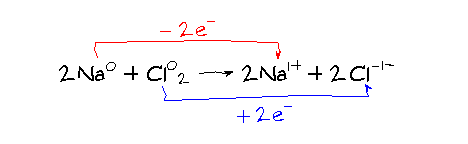
\includegraphics{chemmacros-logo.pdf}
    \par
  } ,
  quote-format = \small\biolinumLF ,
  add-cmds = {
     abinitio, activatechemgreekmapping, AddRxnDesc, anti, aq, aqi,
     ba, bond, bridge,
    cd, ch, changechemgreeksymbol, charrow, chcpd, chemabove, chemalpha,
      chembeta, chemgamma, chemdelta, chemDelta, chemformula@bondlength,
      ChemModule,
      chemomega, chemphi, chemPhi, chemsetup, chlewis, chname , cip, cis, ch,
      CNMR,
    data, DeclareChemArrow, DeclareChemBond, DeclareChemBondAlias,
      DeclareChemCharge, DeclareChemEqConstant, declarechemgreekmapping,
      DeclareChemIUPAC, DeclareChemIUPACShorthand, DeclareChemLatin,
      DeclareChemNMR, DeclareChemNucleophile, DeclareChemPartialCharge,
      DeclareChemParticle, DeclareChemPhase, DeclareChemReaction,
      DeclareChemState,
      delm, delp, Delta, dexter, Dfi,
    el, ElPot, endo, entgegen, Enthalpy, enthalpy, entropy,
    fdelm, fdelp, fmch, fminus, fpch, fplus, fscrm, fscrp,
    gas, ghs, ghslistall, ghspic, gibbs, gram,
    hapto, HNMR, Helmholtz, hydrogen,
    IfChemCompatibilityF, IfChemCompatibilityT, IfChemCompatibilityTF, insitu,
      invacuo, isotope, iupac,
    Ka, Kb, Kw,
    laevus, Lfi, listofreactions, lqd,
    mch, mega, meta, mhName,
    NewChemArrow, NewChemBond, NewChemBondAlias,
      NewChemCharge, NewChemEqConstant, newchemgreekmapping, NewChemIUPAC,
      NewChemIUPACShorthand, NewChemLatin, NewChemMacroset, NewChemNMR,
      NewChemNucleophile, NewChemPartialCharge, NewChemParticle, NewChemPhase,
      NewChemReaction, NewChemState,
      newman, nitrogen, NMR, Nu, Nuc,
    orbital, ortho, ox, OX, oxygen,
    para, pch, per, pH, phase, phosphorus, photon, pKa, pKb, pOH, pos,
      positron, Pot, ProvideChemArrow, ProvideChemBond, ProvideChemCharge,
      ProvideChemEqConstant, ProvideChemIUPAC, ProvideChemIUPACShorthand,
      ProvideChemLatin, ProvideChemNMR, ProvideChemNucleophile,
      ProvideChemPartialCharge, ProvideChemParticle, ProvideChemPhase,
      ProvideChemReaction,
      ProvideChemState, prt,
    Rad, redox, RemoveChemIUPACShorthand, RenewChemArrow, RenewChemBond,
      RenewChemCharge, RenewChemEqConstant, renewchemgreekmapping,
      RenewChemIUPAC, RenewChemIUPACShorthand, RenewChemLatin, RenewChemNMR,
      RenewChemNucleophile, RenewChemPartialCharge, RenewChemParticle,
      RenewChemPhase, RenewChemState,
    Sf, scrm, scrp, second, selectchemgreekmapping, setchemformula,
      ShowChemArrow, ShowChemBond, sld, Sod, state, sulfur,
    trans,
    usechemmodule,
    val,
    zusammen
  } ,
  add-silent-cmds = {
    addplot,
    bottomrule,
    cancel, cdot, ce, cee, celsius, centering, chemfig, chemname, clap,
      cnsetup, code, color, cstack, cstsetup,
    DeclareInstance, DeclareSIUnit, definecolor, draw,
    electronvolt, endtikzpicture,
    footnotesize,
    glqq, grqq,
    hertz, hspace,
    includegraphics, intertext, IUPAC,
    joule,
    kelvin, kilo,
    latin, lc, lewis, Lewis, liquid, ltn,
    metre, midrule, milli, mmHg, mole,
    nano, nicefrac, num, numrange,
    ominus, oplus,
    percent, pgfarrowsdeclarealias, pgfarrowsrenewalias,
    renewtagform, rightarrow,
    sample, scriptscriptstyle, setatomsep, setbondoffset, sfrac, shade,
      shadedraw, shorthandoff, si, SI, sisetup, square, subsection,
    textcolor, textendash, textsuperscript, tikz, tikzpicture, tiny, toprule,
    upbeta, upeta, upgamma, usetikzlibrary,
    volt, vphantom, vspave,
    xspace,
    z@, z@skip
  } ,
  index-setup = { othercode = \footnotesize , level = \section } ,
  makeindex-setup = { columns = 2 , columnsep = 1em }
}

\usepackage{chemfig,booktabs,cancel,varioref,csquotes}

\usepackage[
  a4paper,
  top    = .1\paperheight,
  bottom = .1\paperheight,
  left   = .2\paperwidth,
  right  = .1\paperwidth
]{geometry}


\expandafter\def\csname libertine@figurestyle\endcsname{LF}
\usepackage[libertine]{newtxmath}
\expandafter\def\csname libertine@figurestyle\endcsname{OsF}

\usepackage[biblatex]{embrac}
\ChangeEmph{[}[,.02em]{]}[.055em,-.08em]
\ChangeEmph{(}[-.01em,.04em]{)}[.04em,-.05em]

\usepackage[accsupp]{acro}
\acsetup{
  long-format  = \scshape ,
  short-format = \scshape
}
\DeclareAcronym{ghs}{
  short     = ghs ,
  long      = Globally Harmonized System of Classification and Labelling of
    Chemicals ,
  pdfstring = GHS ,
  accsupp   = GHS
}
\DeclareAcronym{eu}{
  short     = EU ,
  long      = European Union ,
  pdfstring = EU ,
  accsupp   = EU
}
\DeclareAcronym{iupac}{
  short     = iupac ,
  long      = International Union of Pure and Applied Chemistry ,
  pdfstring = IUPAC ,
  accsupp   = IUPAC
}
\DeclareAcronym{UN}{
  short     = un ,
  long      = United Nations ,
  pdfstring = UN ,
  accsupp   = UN
}
\DeclareAcronym{dvi}{
  short     = dvi ,
  long      = device independent file format ,
  pdfstring = DVI ,
  accsupp   = DVO
}
\DeclareAcronym{pdf}{
  short     = pdf ,
  long      = portable document file ,
  pdfstring = PDF ,
  accsupp   = PDF
}
\DeclareAcronym{id}{
  short     = id ,
  long      = identification string ,
  pdfstring = ID ,
  accsupp   = ID
}

\chemsetup{
  modules = {all,polymers} ,
  greek = newtx ,
  formula = chemformula ,
  chemformula/format = \libertineLF
}

\usepackage{siunitx}

\sisetup{
  detect-mode=false,
  mode=text,
  text-rm=\libertineLF
}

\usepackage{filecontents}

\defbibheading{bibliography}{\section{References}}
\addbibresource{\jobname.bib}
\begin{filecontents*}{\jobname.bib}
@book{iupac:greenbook,
  author    = {E. Richard Cohan and Tomislav Cvita\v{s} and Jeremy G. Frey and
    Bertil Holmstr\"om and Kozo Kuchitsu and Roberto Marquardt and Ian Mills and
    Franco Pavese and Martin Quack and J\"urgen Stohner and Herbert L. Strauss and
    Michio Takami and Anders J Thor} ,
  title     = {``Quantities, Symbols and Units in Physical Chemistry'', \acs{iupac}
    Green Book} ,
  shorttitle = {The \acs{iupac} Green Book} ,
  sorttitle = {Quantities, Symbols and Units in Physical Chemistry} ,
  indexsorttitle = {Quantities, Symbols and Units in Physical Chemistry} ,
  edition   = {3rd Edition. 2nd Printing} ,
  year      = {2008} ,
  publisher = {\acs{iupac} \&\ RSC Publishing, Cambridge}
}
@book{iupac:redbook,
  author    = {Neil G. Connelly and Ture Damhus and Richard M. Hartshorn and
    Alan T. Hutton} ,
  title     = {``Nomenclature of Inorganic Chemistry'', \acs{iupac} Red Book} ,
  shorttitle = {The \acs{iupac} Red Book} ,
  sorttitle = {Nomenclature of Inorganic Chemistry} ,
  indexsorttitle = {Nomenclature of Inorganic Chemistry} ,
  year      = {2005} ,
  publisher = { \acs{iupac} \&\ RSC Publishing, Cambridge} ,
  isbn      = {0-85404-438-8}
}
@book{iupac:bluebook,
  author    = {R. Panico and W. H. Powell and J-C. Richer},
  title     = {``Nomenclature of Organic Chemistry, Sections A, B, C, D, E, F,
    and H'', \acs{iupac} Blue Book},
  shorttitle = {The \acs{iupac} Blue Book} ,
  sorttitle = {Nomenclature of Organic Chemistry} ,
  indexsorttitle = {Nomenclature of Organic Chemistry} ,
  edition   = {\mkbibacro{draft}},
  date      = {2004-10-07},
  url       =
  {http://old.iupac.org/reports/provisional/abstract04/BB-prs310305/CompleteDraft.pdf},
  urldate   = {2013-07-07}
}
@misc{eu:ghsystem_regulation,
  author   = {{The European Parliament and The Council of the European Union}},
  sortname = {European Parliament and The Council of the European Union} ,
  title    = {Regulation (EC) No 1272/2008 of the European Parliament and of
    the Council} ,
  subtitle = {on classification, labelling and packaging of substances and
    mixtures, amending and repealing Directives 67/548/EEC and 1999/45/EC, and
    amending Regulation (EC) No 1907/2006} ,
  journal  = {Official Journal of the European Union} ,
  date     = {2008-12-16}
}
@online{unece:ghsystem_implementation,
  author   = {{United Nations Economic Commission for Europe}} ,
  title    = {GHS Implementation} ,
  url      =
    {http://www.unece.org/trans/danger/publi/ghs/implementation_e.html} ,
  urldate  = {2012-03-20} ,
  date     = {2012-03-20}
}
@online{mychemistry:chemmacros-dev,
  author  = {Clemens Niederberger} ,
  title   = {chemmacros development} ,
  url     = {http://www.mychemistry.eu/2015/06/chemmacros-development/} ,
  urldate = {2015-07-16} ,
  date    = {2015-06-14}
}
@online{mychemistry:modular-chemmacros,
  author  = {Clemens Niederberger} ,
  title   = {modular chemmacros} ,
  url     = {http://www.mychemistry.eu/2015/06/modular-chemmacros/} ,
  urldate = {2015-07-16} ,
  date    = {2015-06-08}
}
@online{mychemistry:chemmacros-update-how,
  author  = {Clemens Niederberger} ,
  title   = {a new chemmacros -- but how?} ,
  url     = {http://www.mychemistry.eu/2015/07/a-new-chemmacros-but-how/} ,
  urldate = {2015-07-16} ,
  date    = {2015-07-15}
}  
\end{filecontents*}

\DeclareInstance{xfrac}{chemformula-text-frac}{text}
  {
    scale-factor        = 1 ,
    denominator-bot-sep = -.2ex ,
    denominator-format  = \scriptsize #1 ,
    numerator-top-sep   = -.2ex ,
    numerator-format    = \scriptsize #1 ,
    slash-right-kern    = .05em ,
    slash-left-kern     = .05em
  }

\usetikzlibrary{calc,positioning,decorations.pathmorphing,patterns}

% \newpackagename\chemmacros{chemmacros}
\newcommand*\chemmacrosversion{\csname c_chemmacros_version_number_tl\endcsname}
\newpackagename\chemformula{chemformula}
\newpackagename\ghsystem{ghsystem}
\newpackagename\chemgreek{chemgreek}

\renewcommand*\AmS{\hologo{AmS}}
\newcommand*\TikZ{Ti\textit{k}Z}
\newcommand*\tablehead[1]{\textrm{\bfseries#1}}

% \NewChemPhase{\aqi}{aq,$\infty$}% aqueous solution at infinite dilution
% \NewChemPhase{\cd}{cd}% condensed phase
% \NewChemPhase{\lc}{lc}% liquid crystal

\newname\hensel{Martin Hensel}
\newname\pedersen{Bj\o rn Pedersen}

\newcommand*\iupaccs[3][]{%
  \command{#2}[\quad\iupac{\csuse{#2}}]
    #3\ifblank{#1}{}{\ifblank{#3}{}{ }An alias for this command is \cs{#1}.}%
}

% \undef\module
% \undef\moduleidx
\newidxcmd\chemmodule{\code{#1}}[ (module)]
\newidxcmd\tikzdecoration{\code{#1}}[ (\TikZ\ decoration)]
\AtEndPreamble{%
  \pdfstringdefDisableCommands{%
    \def\chemmodule*#1{\textquotedblleft#1\textquotedblright}%
  }%
}
\newidxcmd\sym{\code{#1}}[ (symbol)]

\makeatletter
\def\cnltx@bash@listings@style{
  language         = bash,
  basicstyle       = {\sourceformat\color{black}},
  % numbers          = left,
  % numberstyle      = \tiny,
  xleftmargin      = 1em,
  numbersep        = .75em,
  gobble           = \cnltx@gobble ,
  columns          = fullflexible,
  literate         =
    {ä}{{\"a}}1
    {ö}{{\"o}}1
    {ü}{{\"u}}1
    {Ä}{{\"A}}1
    {Ö}{{\"O}}1
    {Ü}{{\"U}}1
    {ß}{{\ss}}1 ,
  breaklines       = true,
  keepspaces       = true,
  breakindent      = 1em,
  commentstyle     = \color{comment},
  keywordstyle     = \color{black}\bfseries ,
  stringstyle      = \color{black} ,
  showstringspaces = false ,
  morekeywords     = texdoc
}

\cnltx@expandargs(nx)\lstdefinestyle
  {bash}
  {\expandonce\cnltx@bash@listings@style}

\newcommand*\prompt{}
\patchcmd\lst@NewLine
  {\hbox{}}% search
  {\hbox{}\prompt}% replace
  {}% success
  {}% failure
\newsourcecodeenv[
  code-only,
  sourcecode-options={style=bash},
  pre-code=\def\prompt{\textasciitilde\space\$\space}
]{bash}
\makeatother

\renewcommand*\dictumauthorformat[1]{#1}
\renewcommand*\raggeddictumtext{}

\newcommand*\TF{\textcolor{red}{\uline{\code{\textcolor{cs}{\textit{TF}}}}}}

\makeatletter
\renewenvironment{commands}
  {%
    \cnltx@set@catcode_{12}%
    \let\command\cnltx@command
    \cnltxlist
  }
  {\endcnltxlist}
\newenvironment{tikzcode}
  {%
    \def\arrowtip{\@cnltx@option@item\code}%
    \cnltxlist
  }
  {\endcnltxlist}

\newrobustcmd*\showenv[1]{\beginenv*\code{\{}\env{#1}\code{\}}}
\makeatother

\ExplSyntaxOn
\cs_new_protected:Npn \chemboldchecks #1
  {
    \seq_set_map:NNn \l_tmpa_seq \l__chemmacros_if_bf_seq { \code {##1} }
    \seq_use:Nnnn \l_tmpa_seq {,~} {,~} {~#1~}
  }
\ExplSyntaxOff

\AtBeginDocument{\renewcommand*\reftextfaraway[1]{starting on page~\pageref{#1}}}

\begin{document}

\part{Preliminaries}
\section{Licence, Requirements and \textsc{README}}\label{sec:licence-requ-readme}
\license

\chemmacros\ loads the packages \pkg{expl3}~\cite{bnd:l3kernel} and
\pkg{xparse}~\cite{bnd:l3packages}.  Depending on your usage other packages
will be loaded.  They are mentioned when the corresponding module using the
package is described.

\section{Motivation and Background}\label{sec:motiv-backgr}
This package grew from a small collection of personal helper macros back
in~2010 into a rather big package supporting various different chemical
typesetting tasks.  I hope I have achieved the following points with this
package:
\begin{itemize}
  \item Intuitive usage as far as the syntax of the commands is concerned.
  \item A comprehensive set of macros! If there are any needs you might have
    with respect to typesetting of chemistry which is not supported by this
    package\footnote{Not including needs already solved by other packages such
      as \pkg{chemnum} or \pkg{chemfig}.} then let me know so \chemmacros\ can
    be extended.
  \item The commands shall not only make typesetting easier and faster but
    also the document source more readable with respect to semantics
    (\code{\cs{ortho}-dichlorobenzene} is easier to read and understand than
    \code{\cs*{textit}\Marg{o}-dichlorobenzene}); the first variant in my
    opinion also is more in the spirit of \LaTeXe.
  \item As much customizability as I could think of so every user can adapt
    the commands to his or her own wishes.  Every now and then users have
    wishes which can't be solved with the available options.  Almost always
    I'll add options then.  If you find something please contact me, see
    section~\vref{sec:sugg-bug-reports}.
  \item Default settings that are compliant with the recommendations of the
    \acf{iupac}.
\end{itemize}
Especially the last point in the past needed some pushing from users to get
things right in many places.  If you find anything not compliant with
\ac{iupac} recommendations please contact me, see
section~\vref{sec:sugg-bug-reports}.  Don't forget to add references for the
corresponding \ac{iupac} recommendation.

\section{The Structure of \chemmacros}\label{sec:structure-chemmacros}
\subsection{General Structure}
Since version~5.0 the \chemmacros\ package has a strictly modular
structure\sinceversion{5.0}.  On the one hand this eases maintenance but it
will also allow for easy and quick extension in the future.  In a way it is a
logical consequence from \chemmacros' history: since version~2.0, \ie, since
the fall of~2011 \chemmacros\ already had modular options.

The different modules of \chemmacros\ are divided into two groups:
\begin{enumerate}
  \item Internal modules which provide underlying functionality or basic
    functionality which is not of direct interest from a user perspective but
    might be if you plan to write a module yourself (see
    section~\ref{sec:own-modules} for details).
  \item User modules which provide all the stuff for typesetting.
\end{enumerate}
Both groups each are subdivided into two groups: preloaded modules and modules
which have to be loaded by the programmer (internal modules) or by the
document author (user modules).  Those modules are described in
parts~\ref{part:preloaded-modules} (preloaded modules)
and~\ref{part:additional-modules} (additional modules) of this manual.

The above means that not all functionality is available per default.  If you
want to load \emph{all} modules no matter what then you can say:
\begin{sourcecode}
  \usechemmodule{all}
\end{sourcecode}
or
\begin{sourcecode}
  \chemsetup{modules=all}
\end{sourcecode}
which will load all modules which are part of \chemmacros\ (also see
section~\vref{sec:all-module}). Own modules (see
section~\vref{sec:own-modules}) are \emph{not} loaded through this, though,
and still have to be loaded additionally.

In part~\vref{part:preloaded-modules} the preloaded modules are described,
first the user modules then the internal ones, in
part~\vref{part:additional-modules} the other available modules are described,
again the user modules first.  In each section the modules are described in
an alphabetical order.

\subsection{Using \chemmacros' Options}\label{sec:using-chemm-opti}
Prior to v5.0 \chemmacros\ had quite a number of package options.
\chemmacros\ v5.0 or higher has none!  All of \chemmacros' options are set
using the command
\begin{commands}
  \command{chemsetup}[\oarg{module}\marg{option list}]
    \chemmacros' setup command.
\end{commands}

When an option is described then in the left margin the module the option
belongs to is denoted.  This looks something like this:
\begin{options}
  \keyval{option}{value}\Module{module}\Default
    Description of \option{option}. The module is printed in the left margin.
    The default value to the right is the setting the option has when
    \chemmacros\ is loaded.  This can be an explicit setting but the option
    can also be empty.
  \keychoice{choice-option}{list,of,\default{choices}}\Module{module}\Default{list}
    Description of \option{choice-option}.  A choice option can only be used
    with a predefined list of values. If one of the values is underlined it
    means that the option can be used without value in which case the
    underlined value is chosen.  If no value is underlined then a value
    \emph{has} to be given by the user.
  \keybool{boolean-option}\Module{module}\Default{true}
    Description of \option{boolean-option}.  A boolean option is a choice
    option with exactly the two values \code{true} and \code{false}.  If the
    option is called without value then the underlined value is chosen (which
    is always \code{true} for a boolean option).
\end{options}

An option or list of options belonging to a module \chemmodule{module} can be
set in two ways:
\begin{sourcecode}
  % first possibility:
  \chemsetup[module]{
    option1 = value ,
    option2 = value
  }
  % second possibility:
  \chemsetup{
    module/option1 = value ,
    module/option2 = value
  }
\end{sourcecode}
The second way allows to set options belonging to different modules with one
call of \cs{chemsetup}.

\subsection{Support Package \chemformula}
\chemformula\ provides means of typesetting chemical formulas and reactions.
You will see its macros \cs{ch} and \cs{chcpd} every now and then in this
manual.  When using \chemmacros\ you can consider the \chemformula\
package~\cite{pkg:chemformula} to be loaded as \chemmacros\ makes use of it in
various places.  \chemmacros\ and \chemformula\ are tightly intertwined.
Nevertheless you should be able to use the \pkg{mhchem}~\cite{pkg:mhchem}
package with \chemmacros. Please see section~\vref{sec:using-mhchem} for
details and \latin{caveat}s.  \emph{The recommendation is to use
  \chemformula.}

A historical note: \chemformula\ started as a part of \chemmacros\ in
January~2012.  Since July~2013 it is a completely independent package -- from
\chemformula's point of view.  It is maintained independently and has a manual
of its own.

\subsection{Upgrading from version $<5.0$}
People upgrading from versions $<5.0$ will find that almost everything they
know from earlier versions is the same in versions $\geq5.0$.  But there are
important and \emph{breaking} differences:
\begin{itemize}
  \item \chemmacros\ has no package options any more, all options are set via
    \cs{chemsetup}, also see section~\vref{sec:using-chemm-opti}.
  \item Not all of the features are available per default any more, for some
    the corresponding module has to be loaded explicitly, see
    section~\ref{sec:general-options}.  If suddenly some commands or
    environments seem to be undefined this is the most likely reason.
  \item Some option modules have been renamed (\eg, \module*{iupac} is now
    \module{nomenclature}).  If you experience strange errors when you upgrade
    your document this is the most likely source.
  \item The command family \cs*{NewChem\ldots}, \cs*{RenewChem\ldots} and
    \cs*{DeclareChem\ldots} has a new member \cs*{ProvideChem\ldots}.
  \item In \cs{iupac} the macro \cs*{-} no longer gives a dash with breaking
    point.  Instead \sym*{-} can be used directly\footnote{\cs*{-} is provided
      up to and including v5.2 but is dropped in higher versions.}.
  \item The macro \cs{ox} has another default behaviour (\keyis{pos}{super})
    and the starred version has another effect (\keyis{pos}{top}) than the
    same macro in earlier versions.  Now the default behaviour follows
    \acs{iupac} recommendations.  A second change is that the atom is now
    treated as a \chemformula\ formula.
  \item The syntax of \cs{NewChemReaction} and friends is now different from
    what it used to be.  If you have defined your own reaction environments
    you need to adapt!
  \item \chemmacros\ offers a macro \cs{state} which is similar to but
    different from the earlier macro \cs*{State}.  \cs*{State} is deprecated.
    There are also differences in the syntax of \cs{enthalpy} \vs\ the earlier
    \cs*{Enthalpy}, \cs{entropy} \vs\ \cs*{Entropy} and \cs{gibbs} \vs\
    \cs*{Gibbs}.  The uppercase versions are deprecated. The  macro
    \cs{NewChemState} also has a different syntax now.
  \item At various places in the code improvements and fixes have been made,
    too many to list them here.  You should keep an open eye and first of all
    read the manual closely.
\end{itemize}

\subsection{Compatibility Mode}

\subsubsection{For Users}
It is actually not true that \chemmacros' has no package options any more.  It
has one very important package option:
\begin{options}
  \keychoice{compatibility}{\meta{num},newest,latest}\Default{\chemmacrosversion}
    Let's you specify the version number of \chemmacros\ you want to use.  Any
    version earlier than 5.0 will load v4.7. \ie, the last version before
    \chemmacros\ got its modular structure\footnote{Mostly: the loaded v4.7
      has got a few fixes}.  Not using the option will always load the newest
    version.  Please note that you only can specify the \emph{number} of the
    version.  For a version \enquote{5.2c} you can only set compatibility mode
    \enquote{5.2} but not specify the subrelease.

    Both values \code{newest} and \code{latest} will choose the latest version
    available.
\end{options}

In your document you can check for the compatibility mode.  For the following
functions it is important to understand the rules: \emph{greater} means
\emph{newer}.  The version number is \emph{not} a usual decimal number!  The
syntax for \meta{num} is \meta{major}\code{.}\meta{minor}.  This means that a
version 5.11 is \emph{newer} than a version 5.7!  In the same way \emph{less}
means \emph{older}.  As last example: 5.10 is \emph{newer} (greater) than 5.1.
\begin{commands}
  \command{IfChemCompatibilityTF}[\marg{comp}\marg{num}\marg{true}\marg{false}]
    Checks the value given through the option \option{compatibility} against
    \meta{num} using \meta{comp} and either leaves \meta{true} or \meta{false}
    in the input stream. \meta{comp} can be one of \code{<}, \code{<=},
    \code{=}, \code{>=} or \code{>}.
  \command{IfChemCompatibilityT}[\marg{comp}\marg{num}\marg{true}]
    Checks the value given through the option \option{compatibility} against
    \meta{num} using \meta{comp} and leaves \meta{true} in the input stream if
    the check is logically true.  \meta{comp} can be one of \code{<},
    \code{<=}, \code{=}, \code{>=} or \code{>}.
  \command{IfChemCompatibilityF}[\marg{comp}\marg{num}\marg{false}]
    Checks the value given through the option \option{compatibility} against
    \meta{num} using \meta{comp} and leaves \meta{false} in the input stream if
    the check is logically false.  \meta{comp} can be one of \code{<},
    \code{<=}, \code{=}, \code{>=} or \code{>}.
\end{commands}

A possible usage:
\begin{sourcecode}
  \IfChemCompatibilityT{>=}{5.0}{\usechemmodule{all}}
\end{sourcecode}

Loading \chemmacros\ with \keyis{compatibility}{4.7} also allows to use the
package options from that version:
\begin{sourcecode}
  \usepackage[compatibility=4.7,language=german]{chemmacros}
\end{sourcecode}

\subsubsection{For Module Writers}
For future versions the aim is not to make such breaking changes again.  While
we never know what the future actually will bring \chemmacros\ now has the
tools for tying code to a version number:
\begin{commands}
  \expandable\command*{chemmacros_if_compatiblity:nn}[\TF\ \marg{comp}
  \marg{num} \marg{true} \marg{false}]
    expl3 version of \cs{IfChemCompatibilityTF}.
\end{commands}

In modules one can try adding code for a certain version or range of versions:
\begin{commands}
  \command{ChemCompatibility}[\marg{num} \meta{code} \cs{EndChemCompatibility}]
    Leaves \meta{code} in the input stream if the compatibility version $x$
    given by \option{compatibility} matches \meta{num}
    ($x=\text{\meta{num}}$).
  \command{ChemCompatibilityFrom}[\marg{num} \meta{code} \cs{EndChemCompatibility}]
    Leaves \meta{code} in the input stream if the compatibility version $x$
    given by \option{compatibility} matches \meta{num} or newer.  This means
    \meta{num} is the \emph{oldest} version allowed
    ($x\geq\text{\meta{num}}$).
  \command{ChemCompatibilityTo}[\marg{num} \meta{code} \cs{EndChemCompatibility}]
    Leaves \meta{code} in the input stream if the compatibility version $x$ given
    by \option{compatibility} matches \meta{num} or older.  This means
    \meta{num} is the \emph{newest} version allowed
    ($x\leq\text{\meta{num}}$).
  \command{ChemCompatibilityBetween}[\marg{num1}\marg{num2} \meta{code}
  \cs{EndChemCompatibility}]
    Leaves \meta{code} in the input stream if the compatibility version $x$
    given by \option{compatibility} lies between \meta{num2} and \meta{num2}
    ($\text{\meta{num1}}\leq x\leq\text{\meta{num2}}$).
  \command{EndChemCompatibility}
    This macro \emph{must} end each of the \cs*{ChemCompatibility\ldots}
    macros.
\end{commands}

You may refer to the current version of \chemmacros\ with the following
tokenlists:
\begin{commands}
  \command*{c_chemmacros_date_tl}
    The current release date: \enquote{\csname
      c_chemmacros_date_tl\endcsname}.
  \command*{c_chemmacros_version_major_number_tl}
    The current major version: \enquote{\csname
    c_chemmacros_version_major_number_tl\endcsname}.
  \command*{c_chemmacros_version_minor_number_tl}
    The current minor version: \enquote{\csname
    c_chemmacros_version_minor_number_tl\endcsname}.
  \command*{c_chemmacros_version_number_tl}
    The current version number: \enquote{\csname
    c_chemmacros_version_number_tl\endcsname}.
  \command*{c_chemmacros_version_subrelease_tl}
    The current sub-release: \enquote{\csname
    c_chemmacros_version_subrelease_tl\endcsname}.
  \command*{c_chemmacros_version_tl}
    The current version: \enquote{\csname c_chemmacros_version_tl\endcsname}.
  \command*{c_chemmacros_info_tl}
    The package information: \enquote{\csname
      c_chemmacros_info_tl\endcsname}.
\end{commands}

\section{General Options}\label{sec:general-options}

\chemmacros\ has some core options which don't belong to any of the modules
described in parts~\ref{part:preloaded-modules}
and~\ref{part:additional-modules}.  Those options have no module denoted in
the left margin next to their descriptions and are also set without specifying
a module:
\begin{sourcecode}
  \chemsetup{
    option1 = value ,
    option2 = value
  }
\end{sourcecode}

Two of those options are explained now:
\begin{options}
  \keyval{modules}{comma separated list of module names}\Default
    With this option you can specify which modules you want to load.
    Alternatively you can use \cs{usechemmodule}\marg{comma separated list of
      module names}.
  \keyval{greek}{mapping}\Default
    Explicitly specify which mapping should be used by the \chemgreek\
    package~\cite{pkg:chemgreek}.  For details about what this means please
    refer to section~\vref{sec:greek-module}.
\end{options}

Some internal modules may also define core options, \eg, the \chemmodule{lang}
module, see section~\vref{sec:lang-module}.

\part{The Preloaded Modules}\label{part:preloaded-modules}

\section{User Modules}
\subsection{The \chemmodule*{acid-base} Module}\label{sec:acid-base-module}

Easy representation of \pH, \pKa \ldots
\begin{commands}
  \command{pH} \pH
  \command{pOH} \pOH
  \command{Ka} \Ka, depends on language settings, see
    section~\vref{sec:lang-module}.  The translations can be adapted.
  \command{Kb} \Kb
  \command{Kw} \Kw
  \command{pKa}[\oarg{num}] \cs{pKa}: \pKa, \cs{pKa}\Oarg{1}: \pKa[1], depends
    on language settings, see  section~\vref{sec:lang-module}.  The translations
    can be adapted.
  \command{pKb}[\oarg{num}] \cs{pKb}: \pKb, \cs{pKb}\Oarg{1}: \pKb[1]
  \command{p}[\marg{anything}] \eg\ \cs{p}\Marg{\cs{Kw}} \p{\Kw}
\end{commands}

\begin{example}[side-by-side]
  \Ka\ \Kb\ \pKa\ \pKa[1] \pKb\ \pKb[1]
\end{example}

\begin{cnltxquote}[{\citetitle{iupac:greenbook} \cite[][p.\,103]{iupac:greenbook}}]
 The operator \p{} \textelp{} shall be printed in Roman type.
\end{cnltxquote}

There is one option which changes the style the \p{} is typeset, other options
allow to change the subscript of the constants:
\begin{options}
  \keychoice{p-style}{italics,slanted,upright}\Module{acid-base}\Default{upright}
    Set the style of the \p{} operator.
  \keyval{K-acid}{text}\Module{acid-base}\Default{\cs{ChemTranslate}\Marg{K-acid}}
    The subscript to \cs{Ka} and \cs{pKa}.
  \keyval{K-base}{text}\Module{acid-base}\Default{\cs{ChemTranslate}\Marg{K-base}}
    The subscript to \cs{Kb} and \cs{pKb}.
  \keyval{K-water}{text}\Module{acid-base}\Default{\cs{ChemTranslate}\Marg{K-water}}
    The subscript to \cs{Kw}.
  \keyval{eq-constant}{text}\Module{acid-base}\Default{K}
    The\sinceversion{5.4} symbol of the constants.
\end{options}
\begin{example}
  \pH, \pKa \par
  \chemsetup[acid-base]{p-style=slanted} \pH, \pKa \par
  \chemsetup[acid-base]{p-style=italics} \pH, \pKa
\end{example}

As you can see the default subscripts of \cs{Kw}, \cs{Ka} and \cs{Kb} are
lowercase letters.  The literature is inconclusive about if this is the right
way or if uppercase letters should be preferred.  In textbooks the uppercase
variant usually seems to be used while journals seem to prefer the lowercase
variant.  \chemmacros' default follows the usage in
\citetitle{iupac:greenbook}~\cite{iupac:greenbook}.  If you want to change
this you have two possibilities:

\begin{example}
  % this works only in the preamble:
  % \DeclareTranslation{English}{K-acid}{\mathrm{A}}% use your language here
  % alternative:
  \chemsetup{acid-base/K-acid=\mathrm{A}}% overwrites language dependent settings
  \pKa
\end{example}

The\sinceversion{5.4} constants \Ka, \Kb, and \Kw\ were defined using the
following commands:
\begin{commands}
  \command{NewChemEqConstant}\marg{cs}\marg{name}\marg{subscript}
    Define the constant \meta{cs} with the name \meta{name} and the subscript
    \meta{subscript}.  This also defines the default translation with the key
    \meta{name} using \meta{subscript} as fallback translation (see
    section~\vref{sec:lang-module} for details).  It also defines the option
    \meta{name} for setting the subscript.
  \command{RenewChemEqConstant}\marg{cs}\marg{name}\marg{default appearance}
    The same as \cs{NewChemEqConstant} but renews an existing command.
  \command{DeclareChemEqConstant}\marg{cs}\marg{name}\marg{default appearance}
    The same as \cs{NewChemEqConstant} but overwrites existing commands.
  \command{ProvideChemEqConstant}\marg{cs}\marg{name}\marg{default appearance}
    The same as \cs{NewChemEqConstant} but doesn't throw an error if \meta{cs}
    already exists.
\end{commands}

This is how \cs{Ka} is defined:
\begin{sourcecode}
  \NewChemEqConstant \Ka {K-acid}  { \mathrm{a} }
\end{sourcecode}

\subsection{The \chemmodule*{charges} Module}\label{sec:charges-module}

The \chemmodule{charges} module loads the module \chemmodule{chemformula}.

\subsubsection{Charge Symbols}
\begin{commands}
  \command{fplus} \fplus\ formal positive charge
  \command{fminus} \fminus\ formal negative charge
  \command{scrp} \scrp\ scriptstyle positive charge (\eg, for usage in
    \pkg{chemfig}'s~\cite{pkg:chemfig} formulas).
  \command{scrm} \scrm\ scriptstyle negative charge (\eg, for usage in
    \pkg{chemfig}'s formulas).
  \command{fscrp} \fscrp\ scriptstyle formal positive charge (\eg, for usage
    in \pkg{chemfig}'s formulas).
  \command{fscrm} \fscrm\ scriptstyle formal negative charge (\eg, for usage
    in \pkg{chemfig}'s formulas).
  \command{fsscrp} \fsscrp\ scriptscriptstyle formal positive charge (\eg, for
    usage in \pkg{chemfig}'s formulas).
  \command{fsscrm} \fsscrm\ scriptscriptstyle formal negative charge (\eg, for
    usage in \pkg{chemfig}'s formulas).
\end{commands}

\subsubsection{Ion Charges}\label{sec:ion-charges}
Simple displaying of (real) charges.  It is worth noting that these commands
really are relicts from a time when \chemmacros\ tried hard to be compliant
with \pkg{mhchem} and \chemformula\ didn't exist, yet.  They are still
provided for backwards compatibility but \emph{my recommendation is to use}
\cs{ch} (see the documentation of the \chemformula\
package~\cite{pkg:chemformula}) \emph{and forget about these commands:}
\begin{commands}
  \command{pch}[\oarg{number}]
    positive charge
  \command{mch}[\oarg{number}]
    negative charge
  \command{fpch}[\oarg{number}]
    formal positive charge
  \command{fmch}[\oarg{number}]
    formal negative charge
\end{commands}
\begin{example}[side-by-side]
  A\pch\ B\mch[3] C\fpch[2] D\fmch
\end{example}

\subsubsection{Partial Charges and Similar Stuff}\label{sec:part-charg-simil}

The next ones probably are seldomly needed but nevertheless useful:
\begin{commands}
  \command{delp} \delp\ partial positive charge
  \command{delm} \delm\ partial negative charge
  \command{fdelp} \fdelp\ partial formal positive charge
  \command{fdelm} \fdelm\ partial formal negative charge
\end{commands}

These macros for example can be used with the \cs{ox} command (see
section~\vref{sec:redox-module}) or with the \pkg{chemfig} package:
\begin{example}
  \chemsetup{
    charges/circled = all,
    redox/parse     = false,
    redox/pos       = top
  }
  \ch{"\ox{\delp,H}" -{} "\ox{\delm,Cl}"} \hspace*{1cm}
  \chemfig{\chemabove[3pt]{\lewis{246,Br}}{\delm}-\chemabove[3pt]{H}{\delp}}
\end{example}

\subsubsection{Charge Options}

\begin{options}
  \keychoice{circled}{formal,\default{all},none}\Module{charges}\Default{formal}
    \chemmacros\ uses two different kinds of charges which indicate the usage
    of real ($+/-$) and formal (\fplus/\fminus) charges.  The option
    \code{formal} distinguishes between them, option \code{none} displays them
    all without circle, option \code{all} circles all.
  \keychoice{circletype}{chem,math}\Module{charges}\Default{chem}
    This option switches between two kinds of circled charge symbols:
    \cs{fplus} \fplus/\cs{fminus} \fminus\ (\code{chem}) and
    \verbcode+$\oplus$+ $\oplus$/\verbcode+$\ominus$+ $\ominus$ (\code{math}).
  \keyval{partial-format}{\LaTeX\ code}\Module{charges}\Default{\cs*{tiny}}
    Code which formats the macros defined with \cs{NewChemPartialCharge} (see
    section~\ref{sec:own-charge-macros}).
\end{options}

\subsubsection{Own Charge Macros}\label{sec:own-charge-macros}
Just in case the existing macros don't fit you needs there are commands for
defining new ones or modifying the existing ones.  These commands define
macros like those described in section~\vref{sec:ion-charges}.

\begin{commands}
  \command{NewChemCharge}[\marg{cs}\marg{charge symbol}]
    Defines a new macro \meta{cs}. Raises an error if \meta{cs} already
    exists.
  \command{RenewChemCharge}[\marg{cs}\marg{charge symbol}]
    Redefines a new macro \meta{cs}. Raises an error if \meta{cs} doesn't
    exist.
  \command{DeclareChemCharge}[\marg{cs}\marg{charge symbol}]
    Defines a macro \meta{cs}.  Silently overwrites \meta{cs} if it exists.
  \command{ProvideChemCharge}[\marg{cs}\marg{charge symbol}]
    Defines a new macro \meta{cs}.  Does nothing if \meta{cs} already exists.
\end{commands}
An example of usage is the definition of the existing ion charge macros:
\begin{sourcecode}
  \NewChemCharge\fpch{\fplus}
  \NewChemCharge\fmch{\fminus}
\end{sourcecode}

These commands define macros like those described in
section~\vref{sec:part-charg-simil}. 
\begin{commands}
  \command{NewChemPartialCharge}[\marg{cs}\marg{charge symbol}]
    Defines a new macro \meta{cs}. Raises an error if \meta{cs} already
    exists.
  \command{RenewChemPartialCharge}[\marg{cs}\marg{charge symbol}]
    Redefines a new macro \meta{cs}. Raises an error if \meta{cs} doesn't
    exist.
  \command{DeclareChemPartialCharge}[\marg{cs}\marg{charge symbol}]
    Defines a macro \meta{cs}.  Silently overwrites \meta{cs} if it exists.
  \command{ProvideChemPartialCharge}[\marg{cs}\marg{charge symbol}]
    Defines a new macro \meta{cs}.  Does nothing if \meta{cs} already exists.
\end{commands}
An example of usage is the definition of the existing partial charge macros:
\begin{sourcecode}
  \NewChemPartialCharge\fdelp{\fplus}
  \NewChemPartialCharge\fdelm{\fminus}
\end{sourcecode}

\subsection{The \chemmodule*{nomenclature} Module}\label{sec:nomenclature-module}

The \chemmodule{nomenclature} module loads the \chemmodule{tikz} module.  It
also loads the package \pkg{scrlfile} which is part of the
\KOMAScript\ bundle~\cite{bnd:koma-script}.

\subsubsection{The \cs*{iupac} Command}

Similar to the \pkg{bpchem} package~\cite{pkg:bpchem} \chemmacros\ provides a
command\footnote{The idea and initial implementation is shamelessly borrowed
  from \pkg{bpchem} by \pedersen.} for typesetting \ac{iupac} names.  Why is
that useful?  \ac{iupac} names can get very long.  So long indeed that they
span over more than two lines, especially in two-column documents.  This means
they must be allowed to be broken more than one time.  This is what the
following command does.
\begin{commands}
  \command{iupac}[\marg{IUPAC name}]
    Inside this command use \sym{\textbar} indicate a breaking point
    \sym{\textasciicircum} as a shortcut for \cs*{textsuperscript}. \sym{-},
    \sym{(} and \sym{)} allow words to be broken while still allow the rest of
    word to be hyphenated, likewise \sym{[} and \sym{]}.
\end{commands}

\begin{example}
  \begin{minipage}{.4\linewidth}
    \iupac{%
      Tetra|cyclo[2.2.2.1^{1,4}]-un|decane-2-dodecyl-%
      5-(hepta|decyl|iso|dodecyl|thio|ester)%
    }
  \end{minipage}
\end{example}

The \cs{iupac} command is more of a semantic command.  In many cases you can
achieve (nearly) the same thing by using \cs*{-} instead of \sym{\textbar},
and \cs*{textsuperscript} instead of \sym{\textasciicircum} without
\cs{iupac}.  There are some important differences, though:
\begin{itemize}
  \item The character \sym{-} inserts a small space before the hyphen and
    removes a small space after it.  Also usually words with hyphens are only
    allowed to break at the hyphen.  Inside \cs{iupac} the hyphen will not
    prevent further hyphenation.  The amount of inserted space can be
    customized.
  \item The character \sym{\textbar} not only prevents ligatures but also
    inserts a small space.  The amount of inserted space can be customized.
  \item The characters \sym{(} and \sym{)} allow the word to be hyphenated and
    don't prevent further hyphenation, likewise \sym{[} and \sym{]}.
  \item \sinceversion{5.3}The character \sym{'} is printed as \cs{chemprime}.
\end{itemize}
\begin{example}[side-by-side]
  \huge\iupac{2,4-Di|chlor|pentan} \par
  2,4-Dichlorpentan
\end{example}
\begin{commands}
  \command{chemprime}
    Prints\sinceversion{5.3} a prime character in superscript position.  It is
    defined as \verbcode+\ensuremath{{}^{\prime}}+.
\end{commands}

The spaces inserted by \sym{-} and \sym{\textbar} can be
customized.
\begin{options}
  \keyval{hyphen-pre-space}{dim}\Module{nomenclature}\Default{.01em}
    Set the space that is inserted before the hyphen set with \sym{-}.
  \keyval{hyphen-post-space}{dim}\Module{nomenclature}\Default{-.03em}
    Set the space that is inserted after the hyphen set with \sym{-}.
  \keyval{break-space}{dim}\Module{nomenclature}\Default{.01em}
    Set the space inserted by \sym{\textbar}.
\end{options}

The command \cs{iupac} serves another purpose, too, however.  Regardless of
the setting of the \option{iupac} option (see below) all the commands
presented in this section are always defined \emph{inside} \cs{iupac}.  Quite
a number of the naming commands have very general names: \cs{meta}, \cs{D},
\cs{E}, \cs{L}, \cs{R}, \cs{S}, \cs{trans} and so forth\footnote{Please read
  section~\vref{sec:one-letter-commands} before you consider using the
  one-letter commands}.  This means they either are predefined already (\cs{L}
\L) or are easily defined by another package or class (the \pkg{cool} package
defines both \cs{D} and \cs{E}, for example).  In order to give you control
which commands are defined in which way, there is the option \option{iupac}:
\begin{options}
  \keychoice{iupac}{auto,restricted,strict}\Module{nomenclature}\Default{auto}
    Take care of how \ac{iupac} naming commands are defined.
\end{options}
It has three modes:
\begin{itemize}
 \item \keyis{iupac}{auto}: if the commands are \emph{not} defined by any
   package or class you're using they are available generally, otherwise only
   \emph{inside} \cs{iupac}.
 \item \keyis{iupac}{restricted}: all naming commands are \emph{only} defined
   inside \cs{iupac}.  If the commands are defined by another package they of
   course have that meaning outside.  They're not defined outside otherwise.
 \item \keyis{iupac}{strict}: \chemmacros\ overwrites any other definition and
   makes the commands available throughout the document.  Of course the
   commands can be redefined (but only in the document body).  They will still
   be available inside \cs{iupac} then.
\end{itemize}
Table~\vref{tab:iupac_modes} demonstrates the different modes.

\begin{table}
  \centering
  \caption{Demonstration of \option*{iupac}'s modes.}\label{tab:iupac_modes}
  \begin{tabular}{lccc}
    \toprule
                              & auto       & restricted & strict \\
    \midrule
      \cs{L}                  & \L         & \L         & \iupac{\L} \\
      \cs{iupac}\Marg{\cs{L}} & \iupac{\L} & \iupac{\L} & \iupac{\L} \\
      \cs{D}                  & \D         & ---        & \D \\
      \cs{iupac}\Marg{\cs{D}} & \iupac{\D} & \iupac{\D} & \iupac{\D} \\
    \bottomrule
  \end{tabular}
\end{table}

\subsubsection{Macros Defined (Not Only) For Usage in \cs*{iupac}}

\paragraph{One-letter Macros}\label{sec:one-letter-commands}
For some of the macros explained in this section one-letter commands are
defined -- with a \latin{caveat} in mind, though: they are not actively
recommended.  One-letter commands seldomly have meaningful names and often
they've also been defined by other packages.  This means they make
collaboration more difficult than it needs to be and are a source for package
conflicts.  \chemmacros\ solves the latter problem by only providing them
inside the argument of \cs{iupac}.  The one exception \chemmacros\ makes is
the command \cs{p} (for things like \pH) which is and will remain an official
command (see section~\vref{sec:acid-base-module}).  For all other one-letter
macros alternatives with more meaningful names exist.

\paragraph{Greek Letters}\label{par:greek_letters}

Greek letters in compound names are typeset upright.  Here are a few examples
for the existing macros:
\begin{commands}
  \command{chemalpha}[\quad\chemalpha]
    Upright lowercase alpha
  \command{chembeta}[\quad\chembeta]
    Upright lowercase alpha
  \command{chemgamma}[\quad\chemgamma]
    Upright lowercase alpha
  \command{chemdelta}[\quad\chemdelta]
    Upright lowercase alpha
\end{commands}
There exist two commands for each of the twenty-four Greek letters: a
lowercase and an uppercase version (\cs{chemalpha} and \cs{chemAlpha}).  Those
commands are actually provided by the \chemgreek\ package.  For more details
read section~\vref{sec:greek-module} and also refer to \chemgreek's
documentation.

There are a number of one-letter commands that some people may find convenient
to use which use above mentioned commands to print Greek letters inside
\cs{iupac}.  They're listed in table~\vref{tab:iupac-greek-shortcuts}.

\begin{table}
  \centering
  \caption{\acs*{iupac} shortcuts for Greek letters.}
  \label{tab:iupac-greek-shortcuts}
  \begin{tabular}{*9l}
    \toprule
      macro &
        \cs{a} & \cs{b} & \cs{g} & \cs{d} &
        \cs{k} & \cs{m} & \cs{n} & \cs{w} \\
    \midrule
      letter &
        \iupac{\a} & \iupac{\b} & \iupac{\g} & \iupac{\d} &
        \iupac{\k} & \iupac{\m} & \iupac{\n} & \iupac{\w} \\
    \bottomrule
  \end{tabular}
\end{table}

\begin{example}
  \iupac{5\chemalpha-androstan-3\chembeta-ol} \par
  \iupac{\chemalpha-(tri|chloro|methyl)-\chemomega
    -chloro|poly(1,4-phenylene|methylene)}
\end{example}

\paragraph{Hetero Atoms and added Hydrogen}

Attachments to hetero atoms and added hydrogen atoms are indicated by italic
letters~\cite{iupac:greenbook}.  \chemmacros\ defines a few macros for the
most common ones.
\begin{commands}
  \iupaccs[H]{hydrogen}{The italic H for hydrogen.}
  \iupaccs[O]{oxygen}{The italic O for oxygen.}
  \iupaccs[N]{nitrogen}{The italic N for nitrogen.}
  \iupaccs[Sf]{sulfur}{The italic S for sulfur.}
  \iupaccs[P]{phosphorus}{The italic P for phosphorus.}
\end{commands}
\begin{example}[side-by-side]
  \iupac{\nitrogen-methyl|benz|amide}
  
  \iupac{3\hydrogen-pyrrole}
  
  \iupac{\oxygen-ethyl hexanethioate}
\end{example}

\paragraph{Cahn-Ingold-Prelog}\label{par:cip}
\begin{commands}
  \command{cip}[\marg{conf}]
    Typeset Cahn-Ingol-Prelog descriptors, \eg: \cs{cip}\Marg{R,S}
    \cip{R,S}. \meta{conf} may be a csv list of entries.
  \iupaccs[R]{rectus}{The rectus descriptor.}
  \iupaccs[S]{sinister}{The sinister descriptor.}
\end{commands}

Both these commands and the entgegen/zusammen descriptors get a small
additional amount of kerning after the closing parenthesis.  This amount can
be changed through the following option:
\begin{options}
  \keyval{cip-kern}{dim}\Module{nomenclature}\Default{.075em}
    Set the amount of kerning after the closing parenthesis.
\end{options}

\paragraph{Fischer}
\begin{commands}
  \iupaccs[D]{dexter}{The dexter descriptor.}
  \iupaccs[L]{laevus}{The laevus descriptor.}
\end{commands}

\paragraph{cis/trans, zusammen/entgegen, syn/anti \& tert}
\begin{itemize}
  \item \cs{cis}   \iupac{\cis} \quad \cs{trans} \iupac{\trans}
  \item \cs{fac}   \iupac{\fac} \quad \cs{mer}   \iupac{\mer}
  \item \cs{sin}   \iupac{\sin} \quad \cs{ter}   \iupac{\ter}
  \item \cs{zusammen} \iupac{\zusammen} \quad \cs{entgegen} \iupac{\entgegen}
  \item \cs{syn}   \iupac{\syn} \quad \cs{anti}  \iupac{\anti}
  \item \cs{tert}  \iupac{\tert}
\end{itemize}
An alias for \cs{entgegen} is \cs{E} and an alias for \cs{zusammen} is
\cs{Z}.

\paragraph{ortho/meta/para}
\begin{center}
    \cs{ortho} \iupac{\ortho} \quad
    \cs{meta}  \iupac{\meta} \quad
    \cs{para}  \iupac{\para}
\end{center}

Although these commands are provided I like to cite
\citetitle{iupac:bluebook}~\cite{iupac:bluebook}:

\begin{cnltxquote}[{\cite[][p.\,90]{iupac:bluebook}}]
  The letters \iupac{\ortho}, \iupac{\meta}, and \iupac{\para} have been used
  in place of \textit{ortho}, \textit{meta}, and \textit{para}, respectively,
  to designate the 1,2-, 1,3-, and 1,4- isomers of disubstituted benzene.
  This usage is strongly discouraged and is not used in preferred \acs{iupac}
  names.
\end{cnltxquote}

\paragraph{Absolute Configuration}
\begin{commands}
  \command{Rconf}[\oarg{letter}]
    \cs{Rconf}: \Rconf \quad \cs{Rconf}\oarg{}: \Rconf[]
  \command{Sconf}[\oarg{letter}]
    \cs{Sconf}: \Sconf \quad \cs{Sconf}\oarg{}: \Sconf[]
\end{commands}

\paragraph{Coordination Chemistry}

\chemmacros\ provides a few commands useful in coordination chemistry:
\begin{commands}
  \command{bridge}[\marg{num}\quad\bridge{3}]
    Denote bridging ligand connection.
  \command{hapto}[\marg{num}\quad\hapto{5}]
    Denote hapticity.
  \command{dento}[\marg{num}\quad\dento{2}]
    Denote denticity.
\end{commands}
\begin{example}
  Ferrocene = \iupac{bis(\hapto{5}cyclo|penta|dienyl)iron} \par
  \iupac{tetra-\bridge{3}iodido-tetrakis[tri|methyl|platinum(IV)]}
\end{example}

Two options allow customization:
\begin{options}
  \keychoice{bridge-number}{sub,super}\Module{nomenclature}\Default{sub}
    Appends the number as a subscript or superscript, depending on the choice.
    The \ac{iupac} recommendation is the subscript~\cite{iupac:redbook}.
  \keybool{coord-use-hyphen}\Module{nomenclature}\Default{true}
    Append a hyphen to \cs{hapto}, \cs{dent} and \cs{bridge} or don't.
\end{options}

\paragraph{Examples}
\begin{example}
  \iupac{\dexter-Wein|s\"aure} =
  \iupac{\cip{2S,3S}-Wein|s\"aure} \par
  \iupac{\dexter-($-$)-Threose} =
  \iupac{\cip{2S,3R}-($-$)-2,3,4-Tri|hydroxy|butanal} \par
  \iupac{\cis-2-Butene} =
  \iupac{\zusammen-2-Butene}, \par
  \iupac{\cip{2E,4Z}-Hexa|diene} \par
  \iupac{\meta-Xylol} =
  \iupac{1,3-Di|methyl|benzene}
\end{example}

\subsubsection{Own \cs*{iupac} Macros And Shorthands}

If you find any commands missing you can define them using
\begin{commands}
  \command{NewChemIUPAC}[\marg{cs}\marg{declaration}]
    Define a new \ac{iupac} command that is in any case defined inside of
    \cs{iupac} regardless if \meta{cs} is defined elsewhere already.
  \command{ProvideChemIUPAC}[\marg{cs}\marg{declaration}]
    Define a new \ac{iupac} command that is in any case defined inside of
    \cs{iupac} regardless if \meta{cs} is defined elsewhere already only if
    the corresponding \ac{iupac} macro is not defined, yet.
  \command{RenewChemIUPAC}[\marg{cs}\marg{declaration}]
    Redefine an existing \ac{iupac} command that is in any case defined inside
    of \cs{iupac} regardless if \meta{cs} is defined elsewhere already.
  \command{DeclareChemIUPAC}[\marg{cs}\marg{declaration}]
    Define a new \ac{iupac} command that is in any case defined inside of
    \cs{iupac} regardless if \meta{cs} is defined elsewhere already.  This
    silently overwrites an existing \ac{iupac} macro definition.
  \command{LetChemIUPAC}[\marg{cs1}\marg{cs2}]
    Defines \meta{cs1} to be an alias of \meta{cs2}.
\end{commands}
A command defined in this way will obey the setting of the option
\option{iupac}.  This means any existing command is only overwritten with
\keyis{iupac}{strict}.  However, \cs{NewChemIUPAC} will \emph{not} change the
definition of an existing \ac{iupac} naming command but issue an error if the
\ac{iupac} naming command already exists.  \cs{DeclareChemIUPAC} \emph{will}
overwrite an existing \ac{iupac} command.
\begin{example}
  \NewChemIUPAC\endo{\textsc{endo}}
  \RenewChemIUPAC\anti{\textsc{anti}}
  \iupac{(2-\endo,7-\anti)-2-bromo-7-fluoro|bicyclo[2.2.1]heptane}
\end{example}

\cs{RenewChemIUPAC} allows you to redefine the existing \ac{iupac} naming
commands.
\begin{example}[side-by-side]
  \iupac{\meta-Xylol} \par
  \RenewChemIUPAC\meta{\textup{m}}
  \iupac{\meta-Xylol}
\end{example}

There's also a way for defining new \ac{iupac} shorthands or changing the
existing ones:
\begin{commands}
  \command{NewChemIUPACShorthand}[\meta{shorthand token}\meta{control sequence}]
    Defines a new \ac{iupac} shorthand.  Inside \cs{iupac} it will be equal to
    using \meta{control sequence}.  This throws an error if \meta{shorthand
      token} is already defined.
  \command{RenewChemIUPACShorthand}[\meta{shorthand token}\meta{control sequence}]
    Redefines an existing \ac{iupac} shorthand.  This throws an error if
    \meta{shorthand token} is not defined, yet.
  \command{DeclareChemIUPACShorthand}[\meta{shorthand token}\meta{control sequence}]
    Defines a new \ac{iupac} shorthand or redefines an existing one.
  \command{ProvideChemIUPACShorthand}[\meta{shorthand token}\meta{control sequence}]
    Provides a new \ac{iupac} shorthand.  Does nothing if \meta{shorthand
      token} is already defined.
  \command{RemoveChemIUPACShorthand}[\meta{shorthand token}]
    Deletes an existing \ac{iupac} shorthand.
\end{commands}

\subsubsection{Latin Phrases}

The package \pkg{chemstyle}~\cite{pkg:chemstyle} provides the command
\cs{latin} to typeset common latin phrases in a consistent way.  \chemmacros\
defines a similar \cs{latin} only if \pkg{chemstyle} has \emph{not} been
loaded and additionally provides these commands:
\begin{center}
  \cs{insitu}   \insitu \quad
  \cs{abinitio} \abinitio \quad
  \cs{invacuo}  \invacuo
\end{center}

\emph{If the package \pkg{chemstyle} has been loaded they are defined using
\pkg{chemstyle}'s \cs{latin} command.  This means that then the appearance
depends on \pkg{chemstyle}'s option \code{abbremph}.}

The commands are defined through
\begin{commands}
  \command{NewChemLatin}[\marg{cs}\marg{phrase}]
    Define a new latin phrase.  Gives an error if \meta{cs} already exists.
  \command{DeclareChemLatin}[\marg{cs}\marg{phrase}]
    Define a new latin phrase.  Silently redefined existing macros.
  \command{RenewChemLatin}[\marg{cs}\marg{phrase}]
    Redefine an existing latin phrase.  Gives an error if \meta{cs} doesn't
    exist.
  \command{ProvideChemLatin}[\marg{cs}\marg{phrase}]
    Define a new latin phrase only if \meta{cs} doesn't exist.
\end{commands}
\begin{example}[side-by-side]
  \NewChemLatin\ltn{latin text}\ltn
\end{example}
If you have \emph{not} loaded \pkg{chemstyle} you can change the appearance
with this option:
\begin{options}
  \keyval{format}{definition}\Module{nomenclature}\Default{\cs*{itshape}}
    Set the format of the latin phrases.
\end{options}

\subsection{The \chemmodule*{particles} Module}\label{sec:particles-module}

The \chemmodule{particles} module loads the modules \chemmodule{charges} and
\chemmodule{chemformula}.

\subsubsection{Provided Particle Macros}
The \chemmodule{particles} defines a number of macros which can be used for
typesetting common particles in the running text.  Most of them don't make
much sense in \pkg{chemformula}~\cite{pkg:chemformula}'s \cs{ch}, though,
which doesn't mean that they can't be used there, of course:
\begin{center}
  \cs{el} \el\ \cs{prt} \prt\ \cs{ntr} \ntr\ \cs{Hyd} \Hyd\ \cs{Oxo} \Oxo\
  \cs{water} \water\ \cs{El} \El\ \cs{Nuc} \Nuc\ \cs{ba} \ba
\end{center}
All of these macros are defined using \pkg{chemformula}'s \cs{chcpd}.  The
details are explained in section~\vref{sec:defin-own-part}.

The macros \cs{Nuc} and \cs{ba} are special:  they have an optional argument
for the following options:
\begin{options}
  \keychoice{elpair}{dots,dash,false}\Module{particles}\Default{false}
    Determine how the electron pair of the nucleophiles is displayed.  The
    electron pair is drawn using \chemformula's \cs{chlewis} macro.
  \keyval{space}{dim}\Module{particles}\Default{.1em}
    Sets\sinceversion{5.3} the space that is inserted between the electron
    pair and the negative charge sign.
\end{options}
Both options can of course also be set with \cs{chemsetup}.

\begin{example}[side-by-side]
  \ba[elpair=dots] \Nuc[elpair=dash]
 
  \chemsetup[particles]{elpair=false}
  \ba\ \Nuc
\end{example}

\subsubsection{Defining Own Particle Macros}\label{sec:defin-own-part}

There are two sets of macros, one for defining particles and one for defining
nucleophiles.
\begin{commands}
  \command{NewChemParticle}[\marg{cs}\marg{formula}]
    Defines a new macro \meta{cs}. \meta{formula} is any valid \chemformula\
    compound.  Raises an error if \meta{cs} already exists.
  \command{RenewChemParticle}[\marg{cs}\marg{formula}]
    Redefines a new macro \meta{cs}. \meta{formula} is any valid \chemformula\
    compound.  Raises an error if \meta{cs} doesn't exist.
  \command{DeclareChemParticle}[\marg{cs}\marg{formula}]
    Defines a macro \meta{cs}. \meta{formula} is any valid \chemformula\
    compound.  Silently overwrites \meta{cs} if it exists.
  \command{ProvideChemParticle}[\marg{cs}\marg{formula}]
    Defines a new macro \meta{cs}. \meta{formula} is any valid \chemformula\
    compound.  Does nothing if \meta{cs} already exists.
\end{commands}
An example of usage is the definition of the existing particle macros:
\begin{sourcecode}
  \NewChemParticle\el {e-}
  \NewChemParticle\prt{p+}
  \NewChemParticle\ntr{n^0}
\end{sourcecode}

The following set defines macros like \cs{Nuc}
\begin{commands}
  \command{NewChemNucleophile}[\marg{cs}\marg{formula}]
    Defines a new macro \meta{cs}. \meta{formula} is any valid \chemformula\
    compound. Note that \meta{formula} will get a trailing negative charge!
    Raises an error if \meta{cs} already exists.
  \command{RenewChemNucleophile}[\marg{cs}\marg{formula}]
    Redefines a new macro \meta{cs}. \meta{formula} is any valid \chemformula\
    compound.  Note that \meta{formula} will get a trailing negative charge!
    Raises an error if \meta{cs} doesn't exist.
  \command{DeclareChemNucleophile}[\marg{cs}\marg{formula}]
    Defines a macro \meta{cs}. \meta{formula} is any valid \chemformula\
    compound.  Note that \meta{formula} will get a trailing negative charge!
    Silently overwrites \meta{cs} if it exists.
  \command{ProvideChemNucleophile}[\marg{cs}\marg{formula}]
    Defines a new macro \meta{cs}. \meta{formula} is any valid \chemformula\
    compound.  Note that \meta{formula} will get a trailing negative charge!
    Does nothing if \meta{cs} already exists.
\end{commands}
An example of usage is the definition of the existing nucleophile macros:
\begin{sourcecode}
  \NewChemNucleophile\Nuc{Nu}
  \NewChemNucleophile\ba {ba}
\end{sourcecode}
A macro defined this way will have an optional argument for the
\option{elpair} option.

\subsection{The \chemmodule*{phases} Module}\label{sec:phases-module}

The \chemmodule{phases} module loads the \chemmodule{chemformula} modul.

\subsubsection{Basics}

These commands are intended to indicate the phase of a compound.
\begin{center}
  \cs{sld} \sld \quad \cs{lqd} \lqd \quad \cs{gas} \gas \quad \cs{aq} \aq
\end{center}
\begin{example}
  \ch{C\sld{} + 2 H2O\lqd{} -> CO2\gas{} + 2 H2\gas}\par
  To make it complete: NaCl\aq.
\end{example}

The \ac{iupac} recommendation to indicate the state of aggregation is to put
it in parentheses after the compound \cite{iupac:greenbook}.  However, you
might want to put it as a subscript which is also very common.

\begin{cnltxquote}[{\citetitle{iupac:greenbook}~\cite[][p.\,54]{iupac:greenbook}}]
  The \textelp{} symbols are used to represent the states of aggregation of
  chemical species.  The letters are appended to the formula in parentheses
  and should be printed in Roman (upright) type without a full stop (period).
\end{cnltxquote}

There are two options to customize the output:
\begin{options}
  \keychoice{pos}{side,sub}\Module{phases}\Default{side}
    Switch the position of the phase indicator.
  \keyval{space}{dim}\Module{phases}\Default{.1333em}
    Change the default spacing between compound a phase indicator if
    \keyis{pos}{side}. A \TeX\ dimension.
\end{options}
\begin{example}
  \chemsetup[phases]{pos=sub}
  \ch{C\sld{} + 2 H2O\lqd{} -> CO2\gas{} + 2 H2\gas}\par
  To make it complete: NaCl\aq.
\end{example}

All those phase commands have an optional argument:
\begin{example}[side-by-side]
  \ch{H2O "\lqd[\SI{5}{\celsius}]"}
\end{example}

There is also a generic phase command:
\begin{commands}
  \command{phase}[\marg{phase}]
    If you need a phase indicator just once or twice.  You can use it to
    denote a phase for which there is no phase command, yet.
\end{commands}

\subsubsection{Define Own Phases}
Depending on the subject of your document you might need to indicate other
states of aggregation.  You can easily define them.
\begin{commands}
  \command{NewChemPhase}[\marg{cs}\marg{symbol}]
    Define a new phase command.  See section~\vref{sec:lang-depend} for a way
    to define language dependent settings.  Gives an error if \meta{cs}
    already exists.
  \command{DeclareChemPhase}[\marg{cs}\marg{symbol}]
    Define a new phase command. See section~\vref{sec:lang-depend} for a way to
    define language dependent settings.  Overwrites previous definitions of
    \meta{cs}.
  \command{RenewChemPhase}[\marg{cs}\marg{symbol}]
    Redefine an existing phase command.  See section~\vref{sec:lang-depend} for
    a way to define language dependent settings.  Gives an error if \meta{cs}
    is not defined.
  \command{ProvideChemPhase}[\marg{cs}\marg{symbol}]
    Define a new phase command.  See section~\vref{sec:lang-depend} for a way
    to define language dependent settings.  Does nothing if \meta{cs} is
    already defined.
\end{commands}

\begin{example}
  % preamble:
  \NewChemPhase\aqi{aq,$\infty$} % aqueous solution at infinite dilution
  \NewChemPhase\cd {cd} % condensed phase
  \NewChemPhase\lc {lc} % liquid crystal
  \ch{NaOH\aqi} \ch{H2O\cd} \ch{U\phase{cr}} \ch{A\lc}\par
  \chemsetup[phases]{pos=sub}
  \ch{NaOH\aqi} \ch{H2O\cd} \ch{U\phase{cr}} \ch{A\lc}
\end{example}

\subsubsection{Language Dependencies}\label{sec:lang-depend}
For each phase command a translation into the custom language can be defined.
If a phase is declared with \cs{NewChemPhase} no translation exists and
for every \pkg{babel} language the literal string is used that was provided
as a definition.  Let's say you define the phase
\begin{sourcecode}
  \NewChemPhase\liquid{l}
\end{sourcecode}
and want to add the German translation ``f\/l''.  Then you could do
\begin{sourcecode}
  \DeclareTranslation{German}{phase-liquid}{f\/l}
\end{sourcecode}
This way, when you use it in a German document using the appropriate
\pkg{babel} option using \cs*{liquid} would correctly translate.  For this the
package \pkg{translations}~\cite{pkg:translations} is used.  The \acs{id}
always is \code{phase-\meta{csname}} where \meta{csname} is the name of the
phase command you defined without leading backslash.

See section~\vref{sec:lang-module} for predefined translations and general
language options of \chemmacros.

\subsection{The \chemmodule*{symbols} Module}\label{sec:symbols-module}

The \chemmodule{symbols} module defines a few symbols chemists need now and
then.  It loads the package \pkg{amstext}~\cite{pkg:amstext}.
\begin{commands}
  \command{transitionstatesymbol}
    This is self-explaining: \transitionstatesymbol
  \command{standardstate}
    Again self-explaining: \standardstate
  \command{changestate}
    The uppercase delta used in \state[superscript=]{H} for example.
\end{commands}

\section{Internal Modules}
\subsection{The \chemmodule*{base} Module}\label{sec:base-module}

The \chemmodule{base} module is the core module of \chemmacros. It defines
some tools which can (and should) be used in other modules.  This means this
section is only interesting for you if you plan to write a module yourself
(see section~\vref{sec:own-modules} for details).

This module requires the packages \pkg{bm}~\cite{pkg:bm}, 
\pkg{amstext}~\cite{pkg:amstext}, and \pkg{etoolbox}~\cite{pkg:etoolbox}.

This module also provides \cs{chemsetup} and the option \option{modules}.

It also provides a number of (expl3) macros which may be used in other
modules. In the macro descriptions below \TF\ denotes that a \code{T}, an
\code{F} and a \code{TF} variant exist.  In case of an expandable conditional
(\expandablesymbol) also the predicate variant is available.
\begin{commands}
  \expandable\command*{chemmacros_if_loaded:nn}[\TF\
  \Marg{package|class} \marg{name} \marg{true} \marg{false}]
    Checks if package (or class) \meta{name} has been loaded. Also works after
    begin document.
  \expandable\command*{chemmacros_if_package_loaded:n}[\TF\ \marg{name}
  \marg{true} \marg{false}]
    Checks if package \meta{name} has been loaded. Also works after begin
    document.
  \expandable\command*{chemmacros_if_class_loaded:n}[\TF\ \marg{name}
  \marg{true} \marg{false}]
    Checks if class \meta{name} has been loaded. Also works after begin
    document.
  \command*{chemmacros_leave_vmode:}
    Equivalent of \cs*{leavevmode}.
  \command*{chemmacros_nobreak:}
    Inserts a penalty of \num{10000}.
  \command*{chemmacros_allow_break:}
    Inserts a penalty of \num{0}.
  \command*{chemmacros_skip_nobreak:N}[ \meta{skip/length variable}]
    Insert a horizontal skip where a linebreak is disallowed.
  \expandable\command*{chemmacros_if_is_int:n}[\TF\ \marg{input} \marg{true}
  \marg{false}]
    Checks if \meta{input} is an integer or something else.
  \command*{chemmacros_if_bold:}[\TF\ \marg{true} \marg{false}]
    Checks if the current font weight is one of \chemboldchecks{or}.
  \command*{chemmacros_bold:n}[ \marg{text}]
    Checks if the current font weight is bold and if yes places \meta{text} in
    \cs*{textbf} if in text mode or in \cs*{bm} if in math mode.  If no
    \meta{text} simply is placed in the input stream as is.
  \command*{chemmacros_text:n}[ \marg{text}]
    Ensures that \meta{text} is placed in text mode.
  \command*{chemmacros_math:n}[ \marg{text}]
    Ensures that \meta{text} is placed in math mode.
  \command*{chemmacros_new_macroset:nnn}[ \marg{name} \marg{arg spec}
  \marg{internal command call}]
    \changedversion{5.3b}A command to define a set of macros
    \cs*{NewChem\meta{name}}, \cs*{RenewChem\meta{name}},
    \cs*{DeclareChem\meta{name}} and \cs*{ProvideChem\meta{name}} where the
    first letter of \meta{name} is converted to uppercase, other letters are
    kept unchanged. \meta{arg spec} is any valid argument specification for
    \pkg{xparse}'s \\
    \cs{DeclareDocumentCommand}~\cite{bnd:l3packages}. \meta{internal command
      call} should be a macro which makes definitions \emph{without} error
    checks, \ie, define new macros or redefine existing ones like \cs*{def}
    does.  This macro just should get the arguments passed on to.  Have a look
    at the example below.
  \command*{chemmacros_new_environment_macroset:nnn}[ \marg{name} \marg{arg spec}
  \marg{internal command call}]
    Like \cs*{chemmacros_new_macroset:nnn} but for environments.
  \command{NewChemMacroset}[\sarg\marg{name}\marg{arg spec}\marg{internal
    command call}]
    A non-expl3 version of \cs*{chemmacros_new_macroset:nnn} for \LaTeXe\
    programmers.  The starred version calls
    \cs*{chemmacros_new_environment_macroset:nnn}.
\end{commands}
This is how the macros \cs{NewChemParticle}, \cs{RenewChemParticle},
\cs{DeclareChemParticle} and \cs{ProvideChemParticle} were defined:
\begin{sourcecode}
  \NewChemMacroset {Particle} {mm}
    { \chemmacros_define_particle:Nn #1 {#2} }
\end{sourcecode}

The following macros strictly speaking are not provided by the
\chemmodule{base} module but this place fits best for their description.
\begin{commands}
  \expandable\command*{chemmacros_if_module_exist:n}[\TF\ \marg{module}
  \marg{true} \marg{false}]
    Checks if a file with the correct name for a module \meta{module} can be
    found.
  \expandable\command*{chemmacros_if_module_loaded:n}[\TF\ \marg{module}
  \marg{true} \marg{false}]
    Checks if the module \meta{module} has already been loaded or not.
  \command*{chemmacros_load_module:n}[ \marg{module}]
    Loads module \meta{module} if it hasn't been loaded, yet.
  \command*{chemmacros_load_modules:n}[ \marg{csv list of modules}]
    Loads every module in \meta{csv list of modules} if they haven't been
    loaded, yet. This is the code level variant of \cs{usechemmodule}.
  \command*{chemmacros_before_module:nn}[ \marg{module} \marg{code}]
    Saves\sinceversion{5.1} \meta{code} and inserts it right before
    \meta{module} is loaded.  If \meta{module} is never loaded then
    \meta{code} is never inserted.  If \meta{module} already is loaded when
    the command is used then \meta{code} also is never inserted.
  \command*{chemmacros_after_module:nn}[ \marg{module} \marg{code}]
    Saves\sinceversion{5.1} \meta{code} and inserts it right after
    \meta{module} is loaded.  If \meta{module} is never loaded then
    \meta{code} is never inserted.  If \meta{module} already is loaded when
    the command is used then \meta{code} is inserted immediately.
\end{commands}

\subsection{The \chemmodule*{chemformula} Module}\label{sec:chemformula-module}

The \chemmodule{chemformula} module loads the \pkg{chemformula}
package~\cite{pkg:chemformula} or the \pkg{mhchem} package~\cite{pkg:mhchem}
and the \pkg{amstext} package~\cite{pkg:amstext}.  It also loads the
\chemmodule{charges} module.

\subsubsection{For Users}

This module provides a general option:
\begin{options}
  \keychoice{formula}{chemformula,mhchem}\Default{chemformula}
    This\sinceversion{5.1} option let's you choose if chemical formula's are
    typeset using \pkg{chemformula}'s \cs{ch} and \cs{chcpd} or \pkg{mhchem}'s
    \cs{ce}.  The corresponding package is loaded.
\end{options}
If you explicitly set this option the corresponding package is loaded
immediately.  Otherwise the option is set at the end of the preamble.

If\sinceversion{5.2} you load either \pkg{mhchem} or \pkg{chemformula} and
haven't set \option{formula} \chemmacros\ will choose the corresponding
package.  If you have loaded both \pkg{mhchem} and \pkg{chemformula}
\chemmacros\ will raise a warning and choose \pkg{chemformula}.  \emph{All
  automatic choices only happen at the end of the preamble}.

\paragraph{Using the \pkg*{chemformula} Package}
If you set \keyis{formula}{chemformula} the \chemmodule{chemformula} module
makes it possible that you can set all \chemformula\ options via the
\cs{chemsetup} command using the module \module{chemformula}, for example:
\begin{sourcecode}
  \chemsetup[chemformula]{format=\sffamily}
\end{sourcecode}

Everywhere where \chemmacros\ typesets chemical formulas \chemformula's macros
\cs{chcpd} or \cs{ch} are used, for example in the reaction environments
provided by the \chemmodule{reactions} module.

\paragraph{Using the \pkg*{mhchem} Package}\label{sec:using-mhchem}
If you set \keyis{formula}{mhchem} the \chemmodule{chemformula} module makes
it possible that you can set all of \pkg{mhchem}'s options via the
\cs{chemsetup} command using the module \module{mhchem}, for example:
\begin{sourcecode}
  \chemsetup[mhchem]{format=\sffamily}
\end{sourcecode}

Everywhere where \chemmacros\ typesets chemical formulas \pkg{mhchem}'s macro
\cs{ce} is used, for example in the reaction environments provided by the
\chemmodule{reactions} module.

There are a few \latin{caveat}s if you use this method:
\begin{itemize}
  \item This method has not been extensively tested, yet.  There may be errors
     and wrong output at unexpected places.
  \item Using this method effectively disables the different values of the
    \module{particles} option \option{elpair} (see
    section~\ref{sec:particles-module}).
  \item The different kinds of formal charges provided by the
    \chemmodule{charges} module (see section~\ref{sec:ion-charges}) are
    disabled.  Formal charges always use the math method now.
  \item There may also be other incompatibilities (\eg, \pkg{mhchem} has it's
    own method of setting upright Greek letters so it may or may not disable
    \chemmacros' mechanism).
\end{itemize}

\subsubsection{For Module Writers}

There's are two macros for module writers:
\begin{commands}
  \command*{chemmacros_chemformula:n}[ \marg{formula}]
    This is only a wrapper for \cs{chcpd} or \cs{ce}.  It is recommended that
    module writers use this macro (or a variant thereof) inside of
    \chemmacros' macros whenever they want to display a chemical formula.
    Writers who prefer traditional \LaTeXe\ programming over expl3 should use
    \cs*{chemmacros@formula}.
  \command*{chemmacros_reaction:n}[ \marg{reaction}]
    This is only a wrapper for \cs{ch} or \cs{ce}.  It is recommended that
    module writers use this macro (or a variant thereof) inside of
    \chemmacros' macros whenever they want to display a chemical reaction.
    Writers who prefer traditional \LaTeXe\ programming over expl3 should use
    \cs*{chemmacros@reaction}.
\end{commands}

\subsection{The \chemmodule*{errorcheck} Module}\label{sec:errorcheck-module}
The\sinceversion{5.2} \chemmodule{errorcheck} module provides some rudimentary
support for giving users more meaningful messages when they use a command or
environment provided by a module that they haven't loaded.

\subsection{The \chemmodule*{greek} Module}\label{sec:greek-module}

The \chemmodule{greek} module loads the \pkg{chemgreek}
package~\cite{pkg:chemgreek}.

This module provides one option:
\begin{options}
  \keyval{greek}{mapping}
    A valid value is any valid \chemgreek\ \meta{mapping}.  \chemmacros\ will
    warn you if no mapping has been chosen or if you are using the
    \code{default} or the \code{var-default} mapping because this means that
    no upright Greek letters are available.
\end{options}
If you load a \chemgreek\ support package which allows an unambiguous choice
of a mapping \chemgreek\ will make this choice automatically.  This means if
you say
\begin{sourcecode}
  \usepackage{upgreek}
  \usepackage{chemmacros}
\end{sourcecode}
then \chemmacros\ will use \pkg{upgreek}'s upright Greek letters.  If you
have
\begin{sourcecode}
  \usepackage{upgreek}
  \usepackage{chemmacros}
  \usepackage{textgreek}
\end{sourcecode}
then no unambiguous choice is possible and you should choose a mapping
yourself, for example:
\begin{sourcecode}
  \usepackage{upgreek}
  \usepackage{chemmacros}
  \usepackage{textgreek}
  \chemsetup{greek=textgreek}
\end{sourcecode}
For further details on mappings please refer to \chemgreek's manual.

\subsection{The \chemmodule*{lang} Module}\label{sec:lang-module}

The \chemmodule{lang} module provides language support for \chemmacros.  It
loads the package \pkg{translations}~\cite{pkg:translations}.

\subsubsection{Information For Users}

This module defines the following option:
\begin{options}
  \keychoice{language}{auto,\meta{language}}\Default{auto}
    If set to \code{auto} \chemmacros\ will detect the language used by
    \pkg{babel}~\cite{pkg:babel} or \pkg{polyglossia}~\cite{pkg:polyglossia}
    automatically, the fallback translation is English and will be used if no 
    translation for the actual language is available.  Any language known to
    the \pkg{translations} package is a valid value for \meta{language}.
\end{options}

The language chosen via \option{language} is used for translation of certain
strings in different places all over \chemmacros.  They are mentioned in the
places when the corresponding function of \chemmacros\ is explained.

Translation is done with the help of the \pkg{translations} package, available
translation keys are listed in section~\vref{sec:avail-transl-keys}.

\subsubsection{Available Translation Keys}\label{sec:avail-transl-keys}

Table~\vref{tab:translation-keys} lists (almost) all keys which are predefined
in \chemmacros.  A translation key is a key which is understood by the
\pkg{translations} package and its commands like \cs*{GetTranslation}.  For
each key at least the English fallback translation is provided, for most also
the German translation is provided.  For a few keys also other translations
are provided.  If you find that a translation for your language is missing you
can provide it in the preamble:
\begin{commands}
  \command*{DeclareTranslation}[\marg{language}\marg{key}\marg{translation}]
    Defines a translation of key \meta{key} for the language \meta{language}.
    No error will be raised if a translation of \meta{key} already exists.
    This command can only be used in the preamble and is defined by the
    \pkg{translations} package.
\end{commands}
If you send me an email (see section~\vref{sec:sugg-bug-reports}) with the
translations for your language I'll gladly add them to the next release of
\chemmacros!

\begin{table}
  \centering
  \caption{Translation keys predefined by \chemmacros.}
  \label{tab:translation-keys}
  \NewDocumentCommand\showtranslation{mm}{%
    \SaveTranslationFor\tmp{#1}{#2}%
    \code{\detokenize\expandafter{\tmp}}%
  }
  \NewDocumentCommand\showtranslations{m}{
    \code{#1} &
    \showtranslation{fallback}{#1} &
    \showtranslation{german}{#1}
  }
 \begin{tabular}{lll}
    \toprule
      \bfseries key & \bfseries fallback translation & \bfseries German \\
    \midrule
      \showtranslations{scheme-name} \\
      \showtranslations{scheme-list} \\
      \showtranslations{K-acid} \\
      \showtranslations{K-base} \\
      \showtranslations{K-water} \\
      \showtranslations{phase-sld} \\
      \showtranslations{phase-lqd} \\
      \showtranslations{phase-gas} \\
      \showtranslations{phase-aq} \\
      \showtranslations{list-of-reactions} \\
      \showtranslations{reaction} \\
    \bottomrule
  \end{tabular}
\end{table}

\subsubsection{Information For Module Writers}

\begin{commands}
  \expandable\command*{chemmacros_translate:n}[ \marg{translation key}]
    Translates the given key to the language which is detected automatically
    or given by the user.  Should be used in \chemmacros' macros instead of
    \pkg{translations}' \cs*{GetTranslation}.
  \command*{l_chemmacros_language_tl}
    A token list variable that holds the language which is used by
    \cs*{chemmacros_translate:n} for translation, \emph{after begin
      document}.
  \command{ChemTranslate}[\marg{translation key}]
    A version of \cs*{chemmacros_translate:n} for those who prefer
    traditional \LaTeXe\ programming over expl3.
\end{commands}

\clearpage

\part{Additional Modules}\label{part:additional-modules}

\section{User Modules}
\subsection{The \chemmodule*{all} \emph{pseudo}-module}\label{sec:all-module}

The \chemmodule{all} module is a pseudo module: it doesn't define any
functionality at all.  It does however load all other modules.  So you can say
\begin{sourcecode}
  \chemsetup{ modules = all }
\end{sourcecode}
to ensure that every module is available.  This \emph{will not} load personal
modules!

\subsection{The \chemmodule*{isotopes} Module}\label{sec:isotopes-module}

The \chemmodule{isotope} module loads the \pkg{elements}
package~\cite{pkg:elements}.  This module defines one user command:
\begin{commands}
  \command{isotope}[\sarg\marg{input}]
    \meta{input} can either be the \emph{symbol} of an element or the
    \emph{name} of an element.  Be aware that \emph{the name is language
      dependent}, refer to the manual of the \pkg{elements} package for
    details.  To be on the safe side use the element symbol.

    \meta{input} can also be comma separated list:
    \cs{isotope}\Marg{\meta{nuc},\meta{symbol}}.  If you leave \meta{nuc} out
    then \cs{isotope} will display the most common isotope.  Otherwise
    \meta{nuc} will be used.  If \meta{nuc} is an isotope unknown to the
    \pkg{elements} package \cs{isotope} will write a warning to the log file.

    The starred variant omits the element number.
\end{commands}

\begin{example}[side-by-side]
  \isotope{C}
  \isotope*{C}
  \isotope{14,C}
  \isotope*{14,C}
\end{example}

As input for the element symbol you can choose any of the elements known to
the \pkg{elements} package.

There are options which allow you to determine how the isotope is printed:
\begin{options}
  \keychoice{format}{super,side}\Module{isotopes}\Default{super}
    Either print the isotope number as superscript or to the right of the
    element symbol.
  \keyval{side-connect}{input}\Module{isotopes}\Default{-}
    Determine what is printed between the element symbol and the isotope
    number if \keyis{format}{side}.
\end{options}

\begin{example}[side-by-side]
  \isotope{C}
  \chemsetup[isotopes]{format=side}
  \isotope{C}
  \chemsetup[isotopes]{side-connect=}
  \isotope{C}
\end{example}

\subsection{The \chemmodule*{mechanisms} Module}\label{sec:mechanisms-module}

The module \chemmodule{mechanisms} loads the package
\pkg{amstext}~\cite{pkg:amstext}.  It provides one macro:

\begin{commands}
  \command{mech}[\oarg{type}]
    Allows to specify the most common reaction mechanisms.
\end{commands}
\meta{type} can have one of the following values:
\begin{commands}
  \command{mech}
    (empty, no opt. argument) nucleophilic substitution \mech
  \command{mech}[\Oarg{1}]
    unimolecular nucleophilic substitution \mech[1]
  \command{mech}[\Oarg{2}]
    bimolecular nucleophilic substitution \mech[2]
  \command{mech}[\Oarg{se}]
    electrophilic substitution \mech[se]
  \command{mech}[\Oarg{1e}]
    unimolecular electrophilic substitution \mech[1e]
  \command{mech}[\Oarg{2e}]
    bimolecular electrophilic substitution \mech[2e]
  \command{mech}[\Oarg{ar}]
    electrophilic aromatic substitution \mech[ar]
  \command{mech}[\Oarg{e}]
    elimination \mech[e]
  \command{mech}[\Oarg{e1}]
    unimolecular elimination \mech[e1]
  \command{mech}[\Oarg{e2}]
    bimolecular elimination \mech[e2]
  \command{mech}[\Oarg{cb}]
    unimolecular elimination \enquote{conjugated base}, \ie, via carbanion
    \mech[cb]
\end{commands}

\subsection{The \chemmodule*{newman} Module}\label{sec:newman-module}
The \chemmodule{newman} module provides a command for drawing Newman
projections.  It loads the \chemmodule{tikz} module.
\begin{commands}
  \command{newman}[\oarg{options}\darg{angle}%
    \Marg{\meta{1},\meta{2},\meta{3},\meta{4},\meta{5},\meta{6}}]
    Create Newman projections.  This command uses \TikZ\ internally.
    \meta{angle} rotates the back atoms counter clockwise with respect to the
    front atoms and is an optional argument.  \meta{1} to \meta{6} are the
    positions, the first three are the front atoms, the last three the back
    atoms.
\end{commands}

\begin{example}
  \newman{} \newman(170){}
  \newman{1,2,3,4,5,6} \newman{1,2,3} \newman{,,,4,5,6}
\end{example}

Several options allow customization:
\begin{options}
  \keyval{angle}{angle}\Module{newman}\Default{0}
    Default angle.
  \keyval{scale}{factor}\Module{newman}\Default{1}
    Scale the whole projection by factor \meta{factor}.
  \keyval{ring}{tikz}\Module{newman}\Default
    Customize the ring with \TikZ\ keys.
  \keyval{atoms}{tikz}\Module{newman}\Default
    Customize the nodes within which the atoms are set with \TikZ\ keys.
  \keyval{back-atoms}{tikz}\Module{newman}\Default
    Explicitly customize the nodes of the back atoms with \TikZ\ keys.
\end{options}

\begin{example}
  \chemsetup[newman]{angle=45} \newman{}
  \newman[scale=.75,ring={draw=blue,fill=blue!20}]{}
\end{example}

\begin{example}
  \chemsetup[newman]{atoms={draw=red,fill=red!20,inner sep=2pt,rounded corners}}
  \newman{1,2,3,4,5,6}
\end{example}

\begin{example}
  \chemsetup[newman]{
    atoms = {draw=red,fill=red!20,inner sep=2pt,rounded corners},
    back-atoms = {draw=blue,fill=blue!20,inner sep=2pt,rounded corners}
  }
  \newman{1,2,3,4,5,6} \newman(170){1,2,3,4,5,6}
\end{example}

\subsection{The \chemmodule*{orbital} Module}\label{sec:orbital-module}
The \chemmodule{orbital} module loads the \chemmodule{tikz} module.  It
provides the following command to create orbitals:
\begin{commands}
  \command{orbital}[\oarg{options}\marg{type}]
    Draw an orbital shape of type \meta{type}.  This command uses \TikZ\
    internally.
\end{commands}

There are the following types available for \meta{type}:
\begin{center}
  \code{s} \quad
  \code{p} \quad
  \code{sp} \quad
  \code{sp2} \quad
  \code{sp3}
\end{center}

\begin{example}
  \orbital{s} \orbital{p} \orbital{sp} \orbital{sp2} \orbital{sp3}
\end{example}

Depending on the type you have different options to modify the orbitals:
\begin{options}
  \keychoice{phase}{+,-}\Module{orbital}\Default{+}
    changes the phase of the orbital (all types)
  \keyval{scale}{factor}\Module{orbital}\Default{1}
    changes the size of the orbital (all types)
  \keyval{color}{color}\Module{orbital}\Default{black}
    changes the color of the orbital (all types)
  \keyval{angle}{angle}\Module{orbital}\Default{0}
    rotates the orbitals with a p contribution counter clockwise (all types
    except \code{s})
  \keybool{half}\Module{orbital}\Default{false}
    displays only half an orbital (only \code{p})
\end{options}

\begin{example}
  \orbital{s} \orbital[phase=-]{s} 
  \orbital{p} \orbital[phase=-]{p}
  \orbital{sp3} \orbital[phase=-]{sp3}
 
  \orbital[angle=0]{p} \orbital[color=red!50]{p}
  \orbital[angle=135,scale=1.5]{p} \orbital[half]{p}
\end{example}

Additionally there are two options, with which the \TikZ\ behaviour can be
changed.
\begin{options}
  \keybool{overlay}\Module{orbital}
    The orbital \enquote{doesn't need space}; it is displayed with the \TikZ\
    option \code{overlay}.
  \keyval{opacity}{num}\Module{orbital}
    The orbital becomes transparent; \meta{value} can have values between
    \code{1} (fully opaque) to \code{0} (invisible).
\end{options}
\begin{example}
  \vspace{7mm}
  \chemsetup[orbital]{
    overlay,
    p/color = black!70
  }
  \setbondoffset{0pt}
  \chemfig{
    ?\orbital{p}
    -[,1.3]{\orbital[phase=-]{p}}
    -[:30,1.1]\orbital{p}
    -[:150,.9]{\orbital[phase=-]{p}}
    -[4,1.3]\orbital{p}
    -[:-150,1.1]{\orbital[phase=-]{p}}?
  }
  \vspace{7mm}
\end{example}

\begin{example}
  \vspace{7mm}
  \setbondoffset{0pt}
  \chemsetup[orbital]{
    overlay ,
    opacity = .75 ,
    p/scale = 1.6 ,
    s/color = blue!50 ,
    s/scale = 1.6
  }
  \chemfig{
    \orbital{s}
    -[:-20]{\orbital[scale=2]{p}}
           {\orbital[half,angle=0]{p}}
           {\orbital[angle=170,half]{p}}
           {\orbital[angle=-150,half]{p}}
    (-[:-150]\orbital{s})-\orbital{s}
  }
  \vspace{1cm}
\end{example}

\subsection{The \chemmodule*{polymers} Module}\label{sec:polymers-module}
The\sinceversion{5.5} \chemmodule{polymers} module loads the
\chemmodule{nomenclature} module.

It defines a number of \ac{iupac} macros for usage inside \cs{iupac} which are
used in polymer chemistry.

\subsubsection{Copolymers}
\begin{commands}
  \iupaccs[co]{copolymer}{unspecified copolymer.}
  \iupaccs[stat]{statistical}{statistical copolymer.}
  \iupaccs[ran]{random}{random copolymer.}
  \iupaccs[alt]{alternating}{alternating copolymer.}
  \iupaccs[per]{periodic}{periodic copolymer.}
  \iupaccs{block}{block copolymer.}
  \iupaccs{graft}{graft copolymer.}
\end{commands}

\subsubsection{Non-linear (Co)Polymers and Polymer Assemblies}
\begin{commands}
  \iupaccs{blend}{The blend qualifier.}
  \iupaccs{comb}{The comb qualifier.}
  \iupaccs[compl]{complex}{The complex qualifier.}
  \iupaccs[cyclo]{cyclic}{The cyclic qualifier.}
  \iupaccs{branch}{The branch qualifier.}
  \iupaccs[net]{network}{The network qualifier.}
  \iupaccs[ipn]{ipnetwork}{The interpenetrating network qualifier.}
  \iupaccs[sipn]{sipnetwork}{The semi-interpenetrating network qualifier.}
  \iupaccs{star}{The star qualifier.}
\end{commands}

\subsection{The \chemmodule*{reactions} Module}\label{sec:reactions-module}
The \chemmodule{reactions} module loads the \chemmodule{chemformula} module
and the \pkg{mathtools} package~\cite{pkg:mathtools}.

\subsubsection{Predefined Environments}

You can use these environments for numbered\ldots
\begin{environments}
  \environment{reaction}
    A single reaction where \chemformula\ code is placed directly in the
    environment body.  A wrapper around the \env*{equation} environment.  The
    environment body is parsed with \cs{ch} or \cs{ce} depending on the value
    of the \option{formula} option, see
    section~\vref{sec:chemformula-module}.
  \environment{reactions}
    Several aligned reactions.  A wrapper around \pkg{amsmath}'s \env*{align}
    environment.  The environment body is parsed with \cs{ch} or \cs{ce}
    depending on the value of the \option{formula} option, see
    section~\vref{sec:chemformula-module}.
\end{environments}

\ldots and their starred versions for unnumbered reactions.
\begin{environments}
  \environment{reaction*}
    A wrapper around the \env*{equation*} environment.  The environment body
    is parsed with \cs{ch} or \cs{ce} depending on the value of the
    \option{formula} option, see section~\vref{sec:chemformula-module}.
  \environment{reactions*}
    A wrapper around \pkg{amsmath}'s \env*{align*} environment.  The
    environment body is parsed with \cs{ch} or \cs{ce} depending on the value
    of the \option{formula} option, see
    section~\vref{sec:chemformula-module}.
\end{environments}

With those environments you can create (un)numbered reaction equations similar
to mathematical equations.

Theses environments use the \env*{equation}/\env*{equation*} environments or
the \env*{align}/\env*{align*} environments, respectively, to display the
reactions.

\begin{example}
  Reaction with counter:
  \begin{reaction}
    A -> B
  \end{reaction}
\end{example}

\begin{example}
  Reaction without counter:
  \begin{reaction*}
    C -> D
  \end{reaction*}
\end{example}

\begin{example}
  Several aligned reactions with counter:
  \begin{reactions}
    A     &-> B + C \\
    D + E &-> F
  \end{reactions}
\end{example}

\begin{example}
  Several aligned reactions without counter:
  \begin{reactions*}
    G     &-> H + I \\
    J + K &-> L
  \end{reactions*}
\end{example}

If you want to change the layout of the counter tags, you can use

\begin{commands}
  \command*{renewtagform}[\marg{tagname}\oarg{format}\marg{right delimiter}\marg{left
  delimiter}]
    Provided by the \pkg{mathtools} package.
\end{commands}

\begin{example}
  \renewtagform{reaction}[R \textbf]{[}{]}
  \begin{reaction}
    H2O + CO2 <<=> H2CO3
  \end{reaction}
\end{example}

The use of \AmS math's \cs{intertext} is possible:
\begin{example}
  \begin{reactions}
    A + 2 B &-> 3 C + D "\label{rxn:test}"
    \intertext{Some text in between aligned reactions}
    3 E + F &<=> G + 1/2 H
  \end{reactions}
  See reaction~\ref{rxn:test}.
\end{example}

% \emph{You should not use \cs{mch} and its relatives inside the \env{reaction}
%   environments.}

\subsubsection{Own Reactions}
You can create new types of reactions with the command:
\begin{commands}
  \command{NewChemReaction}[\marg{name}\oarg{number of arguments}\marg{math name}]
    \meta{name} will be the name of the new chem environment. \meta{math name} is
    the underlying math environment.  Gives an error if \meta{name} already
    exists.
  \command{RenewChemReaction}[\marg{name}\oarg{number of arguments}\marg{math name}]
    \meta{name} is the name of the renewed chem environment. \meta{math name} is
    the underlying math environment.  Gives an error if \meta{name} does not exist.
  \command{DeclareChemReaction}[\marg{name}\oarg{number of arguments}\marg{math name}]
    \meta{name} will be the name of the chem environment. \meta{math name} is
    the underlying math environment.
  \command{ProvideChemReaction}[\marg{name}\oarg{number of arguments}\marg{math name}]
    \meta{name} will be the name of the new chem environment. \meta{math name} is
    the underlying math environment.  The new environment is only defined if
    it doesn't exist, yet.
\end{commands}

\begin{sourcecode}
  \NewChemReaction{reaction}  {equation}
  \NewChemReaction{reaction*} {equation*}
  \NewChemReaction{reactions} {align}
  \NewChemReaction{reactions*}{align*}
\end{sourcecode}

Let's suppose, you'd like to have the alignment behaviour of the \env{alignat}
environment for \chemformula\ reactions.  You could do the following:

\begin{sourcecode}
  \NewChemReaction{reactionsat}[1]{alignat}
\end{sourcecode}

With this the \env{reactionsat} environment is defined.
\begin{example}
  \NewChemReaction{reactionsat}[1]{alignat}
  \NewChemReaction{reactionsat*}[1]{alignat*}
  \begin{reactionsat}{3}
    A     &-> B     &&-> C     &&-> D \\
    aaaaa &-> bbbbb &&-> ccccc &&-> ddddd
  \end{reactionsat}
  \begin{reactionsat*}{2}
    A     &-> B     & C            &-> D  \\
    aaaaa &-> bbbbb &\quad{} ccccc &-> ddddd
  \end{reactionsat*}
\end{example}

\subsubsection{List of Reactions}

The \chemmodule{reactions} module also provides a command to display a list of
the reactions created with the \env{reaction} environment.
\begin{commands}
  \command{listofreactions}
    Print a list of reactions.
\end{commands}
\begin{example}
  \listofreactions
\end{example}

The output of this list can be modified by two options:
\begin{options}
  \keyval{list-name}{name of the
    list}\Module{reactions}\Default{\cs*{ChemTranslate}\Marg{{list-of-reactions}}}
    Let's you set the name of the list manually.  The default name is language
    dependent, see section~\vref{sec:lang-module}.
  \keyval{list-entry}{prefix to each
    entry}\Module{reactions}\Default{\cs*{ChemTranslate}\Marg{reaction}}
    Let's you set a prefix to each list entry.  The default name is language
    dependent, see section~\vref{sec:lang-module}.
  \keyval{list-heading-cmd}{code}\Module{reactions}\Default{\cs*{section}\sarg\Marg{\#1}}
    The\sinceversion{5.2} macro that is called at the beginning of the list.
    Inside of \meta{code} \code{\#1} refers to the actual heading of the list.
    The default setting is not entirely true: if a macro \cs*{chapter} is
    defined \code{\cs*{chapter}\sarg\Marg{\#1}} is used.
\end{options}
Instead of using the option \option{list-name} you also could redefine
\cs{reactionlistname}.

The list lists all reactions with a number and disregards reactions without
number.  All reaction environments without star have an optional argument
which let's you add a description (or caption) for the entry in the list.
\begin{example}
  \begin{reaction}[Autoprotolyse]
    2 H2O <<=> H3O+ + OH-
  \end{reaction}
\end{example}

If you use the \env{reactions} environment this will not work, though.  In
this case you can use
\begin{commands}
  \command{AddRxnDesc}[\marg{description}]
    Add a description to a reaction.
\end{commands}

\begin{example}
  \begin{reactions}
    "\chlewis{0.}{Cl}" + CH4  &
      -> HCl + "\chlewis{180.}{C}" H3 \AddRxnDesc{first~step~of~chain} \\
    "\chlewis{180.}{C}" H3 + Cl2 &
      -> CH3Cl + "\chlewis{0.}{Cl}" \AddRxnDesc{second~step~of~chain}
  \end{reactions}
\end{example}

\subsection{The \chemmodule*{redox} Module}\label{sec:redox-module}

The \chemmodule{redox} module loads the modules \chemmodule{tikz} and
\chemmodule{xfrac}. It also loads the packages
\pkg{mathtools}~\cite{pkg:mathtools} and \pkg{relsize}~\cite{pkg:relsize}.

\subsubsection{Oxidation Numbers}\label{sec:oxidation-numbers}

Regarding the typesetting of oxidation numbers
\citetitle{iupac:greenbook}~\cite{iupac:greenbook} says the following:
\begin{cnltxquote}[{\cite[][p.\,50]{iupac:greenbook}}]
  Oxidation numbers are denoted by positive or negative Roman numerals or by
  zero \textelp{}

  \textit{Examples}\quad \ox{7,Mn}, \ox[pos=side]{7,manganese}, \ox{-2,O},
  \ox{0,Ni}
\end{cnltxquote}

The following command is provided to set oxidation numbers:
\begin{commands}
  \command{ox}[\sarg\oarg{options}\Marg{\meta{number},\meta{atom}}]
    Places \meta{number} as right superscript to \meta{atom}; \meta{number}
    has to be a (rational) number!  \meta{atom} is treated as a \chemformula\
    formula, like it would be in \cs{chcpd}.
\end{commands}

\begin{example}
  \ox{+1,Na}, \ox{2,Ca}, \ox{-2,S}, \ox{-1,F}
\end{example}

There are a number of options that can be used to modify the typeset result:
\begin{options}
  \keybool{parse}\Module{redox}\Default{true}
    When \code{false} an arbitrary entry can be used for \code{<number>}.
  \keybool{roman}\Module{redox}\Default{false}
    Switches from roman to arabic numbers.
  \keychoice{pos}{top,super,side}\Module{redox}\Default{super}
    \code{top} places \meta{number} above \meta{atom}, \code{super} to the
    upper right as superscript and \code{side} to the right and inside
    brackets.  Both \code{super} and \code{side} follow \ac{iupac}
    recommendation, \code{top} does not!
  \keybool{explicit-sign}\Module{redox}\Default{false}
    Shows the $+$ for positiv numbers and the $\pm$ for $0$.
  \keybool{explizit-zero-sign}\Module{redox}\Default{true}
    Only\sinceversion{5.4} if both \option{explicit-sign} and
    \option{explicit-zero-sign} are set to \code{true} $\pm0$ will be
    printed.
  \keychoice{decimal-marker}{comma,point}\Module{redox}\Default{point}
    Choice for the decimal marker for formal oxidation numbers like \ox{1.2,X}.
  \keychoice{align}{center,right}\Module{redox}\Default{center}
    Center the oxidation number relative to the atom or right-align it.
  \keyval{side-connect}{code}\Module{redox}\Default{\cs*{,}}
    Code that is inserted between atom and oxidation number if
    \keyis{pos}{side} is used.
  \keyval{text-frac}{cs}\Module{redox}\Default{\cs{chemfrac}\Oarg{text}\Marg{\#1}\Marg{\#2}}
    The fraction macro that is used for fractions if \keyis{pos}{side} is
    used.  \meta{cs} must be a macro that takes two mandatory arguments, the
    first for the numerator and the second for the denominator.
  \keyval{super-frac}{cs}\Module{redox}\Default{\cs{chemfrac}\Oarg{superscript}%
    \Marg{\#1}\Marg{\#2}}
    The fraction macro that is used for fractions if \keyis{pos}{top} or
    \keyis{pos}{super} is used.  \meta{cs} must be a macro that takes two
    mandatory arguments, the first for the numerator and the second for the
    denominator.
\end{options}

\begin{example}[side-by-side]
  \ox[roman=false]{2,Ca} \ox{2,Ca} \\
  \ox[pos=top]{3,Fe}-Oxide \\
  \ox[pos=side]{3,Fe}-Oxide \\
  \ox[parse=false]{?,Mn} \\
  \ox[pos=top,align=right]{2,Ca}
\end{example}

The \keyis{pos}{top} variant also can be set with the shortcut \cs{ox}\sarg:
\begin{example}[side-by-side]
  \ox{3,Fe} \ox*{3,Fe}
\end{example}

Using the \option{explicit-sign} option will always show the sign of the
oxidation number:
\begin{example}
  \chemsetup[redox]{explicit-sign = true}
  \ox{+1,Na}, \ox{2,Ca}, \ox{-2,S}, \ch{"\ox{0,F}" {}2}
\end{example}

\begin{example}
  \chemsetup[redox]{pos=top}
  Compare \ox{-1,O2^2-} to \ch{"\ox{-1,O}" {}2^2-}
\end{example}

Sometimes one might want to use formal oxidation numbers like \num{.5} or
\chemfrac{1}{3}:
\begin{example}[side-by-side]
  \chemsetup[redox]{pos=top}
  \ox{.5,Br2}
  \ch{"\ox{1/3,I}" {}3+}

  \chemsetup[redox]{pos=side}
  \ox{1/3,I3+}
\end{example}

The fraction is displayed with the help of the \pkg{xfrac}
package~\cite{bnd:l3packages}.  For more details on how \chemmacros\ uses it
read section~\vref{sec:xfrac-module}.

\subsubsection{Redox Reactions}\label{sec:redox-reactions}

\chemmacros\ provides two commands to visualize the transfer of electrons in
redox reactions.  Both commands are using \TikZ.
\begin{commands}
  \command{OX}[\Marg{\meta{name},\meta{atom}}]
    Label \meta{atom} with the label \meta{name}.
  \command{redox}[\Darg{\meta{name1},\meta{name2}}\oarg{tikz}\oarg{num}\marg{text}]
    Connect two \meta{atom}s previously labelled with \cs{OX}.  Only the first
    argument \Darg{\meta{name1},\meta{name2}} is required, the others are all
    optional.
\end{commands}

\cs{OX} places \meta{atom} into a node, which is named with \meta{name}.  If
you have set two \cs{OX}, they can be connected with a line using \cs{redox}.
To do so the names of the two nodes that are to be connected are written in
the round braces.  Since \cs{redox} draws a \code{tikzpicture} with options
\code{remember picture,overlay}, the document needs to be \emph{compiled at
  least two times}.

\begin{example}
  \vspace{7mm}
  \OX{a,Na} $\rightarrow$ \OX{b,Na}\pch\redox(a,b){oxidation}
\end{example}

This line can be customized using \TikZ\ keys in \oarg{tikz}:
\begin{example}
  \vspace{7mm}
  \OX{a,Na} $\rightarrow$ \OX{b,Na}\pch\redox(a,b)[->,red]{ox}
\end{example}

With the argument \oarg{num} the length of the vertical parts of the line can
be adjusted.  The default length is \code{.6em}.  This length is multiplied
with \meta{num}.  If you use a negative value the line is placed \emph{below}
the text.
\begin{example}
  \vspace{7mm}
  \OX{a,Na} $\rightarrow$ \OX{b,Na}\pch
  \redox(a,b)[->,red]{ox}
  \redox(a,b)[<-,blue][-1]{red}
  \vspace{7mm}
\end{example}

The default length of the vertical lines can be customized with the option
\begin{options}
  \keyval{dist}{dim}\Module{redox}\Default{.6em}
    A \TeX\ dimension.
\end{options}

\begin{example}
  \vspace{7mm}
  \chemsetup{redox/dist=1em}
  \OX{a,Na} $\rightarrow$ \OX{b,Na}\pch\redox(a,b)[->,red]{ox}
\end{example}

\begin{options}
  \keyval{sep}{dim}\Module{redox}\Default{.2em}
    The option can be used to change the distance between the atom and the
    beginning of the line.
\end{options}

\begin{example}
  \vspace{7mm}
  \chemsetup{redox/sep=.5em}
  \OX{a,Na} $\rightarrow$ \OX{b,Na}\pch\redox(a,b)[->,red]{ox}
\end{example}

\paragraph{Examples}
\begin{example}
  \vspace{7mm}
  \ch{
    2 "\OX{o1,Na}" + "\OX{r1,Cl}" {}2
    ->
    2 "\OX{o2,Na}" {}+ + 2 "\OX{r2,Cl}" {}-
  }
  \redox(o1,o2){\small OX: $- 2\el$}
  \redox(r1,r2)[][-1]{\small RED: $+ 2\el$}
  \vspace{7mm}
\end{example}

\begin{example}
  \vspace{7mm}
  \ch{
    2 "\OX{o1,\ox*{0,Na}}" + "\OX{r1,\ox*{0,Cl}}" {}2
    ->
    2 "\OX{o2,\ox*{+1,Na}}" {}+ + 2 "\OX{r2,\ox*{-1,Cl}}" {}-
  }
  \redox(o1,o2){\small OX: $- 2\el$}
  \redox(r1,r2)[][-1]{\small RED: $+ 2\el$}
  \vspace{7mm}
\end{example}

\begin{example}
  \vspace{14mm}
  \ch{
    2 "\OX{o1,\ox*{0,Na}}" + "\OX{r1,\ox*{0,Cl}}" {}2
    ->
    2 "\OX{o2,\ox*{+1,Na}}" {}+ + 2 "\OX{r2,\ox*{-1,Cl}}" {}-
  }
  \redox(o1,o2)[draw=red,->][3.33]{\small OX: $- 2\el$}
  \redox(r1,r2)[draw=blue,->]{\small RED: $+ 2\el$}
\end{example}

\begin{example}
  \vspace{7mm}
  \ch{
    2 "\OX{o1,\ox*{0,Na}}" + "\OX{r1,\ox*{0,Cl}}" {}2
    -> 2 "\OX{o2,\ox*{+1,Na}}" {}+ + 2 "\OX{r2,\ox*{-1,Cl}}" {}-
  }
  \redox(o1,o2)[green,-stealth]{\small OX}
  \redox(r1,r2)[purple,-stealth][-1]{\small RED}
  \vspace{7mm}
\end{example}

\subsection{The \chemmodule*{scheme} Module}\label{sec:scheme-module}

The \chemmodule{scheme} module loads the \pkg{chemnum}
package~\cite{pkg:chemnum} and defines a floating environment
\showenv{scheme}.  That is, it \emph{only} defines this float if no
environment \env{scheme} exists at the end of the preamble.  The module checks
for different available float defining methods, in \emph{this} order:
\begin{itemize}
  \item If the current class is a \KOMAScript\ class \cs*{DeclareNewTOC} will
    be used.
  \item If the current class is \cls{memoir}, \cls{memoir}'s methods are used.
  \item If the package \pkg{tocbasic} has been loaded \cs*{DeclareNewTOC} will
    be used.
  \item If the package \pkg{newfloat} has been loaded
    \cs*{DeclareFloatingEnvironment} will be used.
  \item \sinceversion{5.1}If the package \pkg{floatrow} has been loaded its
    method will be used.
  \item If the package \pkg{float} has been loaded its method will be used.
  \item If neither of the above the \enquote{manual} method is used.  This
    means the environment is defined the same way like \env*{figure} is
    defined in the \cls*{article} class or the \cls*{book} class, depending if
    \cs*{chapter} is defined or not.
\end{itemize}

The list name and the caption name both are translated to the language
specified according to the \option{lang} option and the provided translations,
see section~\vref{sec:lang-module} for details. If you want to manually change
them then redefine these macros after begin document:
\begin{commands}
  \command{listschemename}
    The name of the list of schemes.
  \command{schemename}
    The name used in captions.
\end{commands}
The list of schemes is printed as expected with
\begin{commands}
  \command{listofschemes}
\end{commands}

\subsection{The \chemmodule*{spectroscopy} Module}\label{sec:spectroscopy-module}

The \chemmodule{spectroscopy} module loads the \chemmodule{chemformula} module
and the \pkg{siunitx} package~\cite{pkg:siunitx}.

\subsubsection{The \cs*{NMR} Command}

When you're trying to find out if a compound is the one you think it is often
NMR spectroscopy is used.  The experimental data are typeset similar to this:
\begin{center}
  \NMR(400)[CDCl3] = \num{1.59}
\end{center}
The \chemmodule{spectroscopy} module provides a command which simplifies the
input.

\begin{commands}
  \command{NMR}[\sarg\Marg{\meta{num},\meta{element}}%
    \Darg{\meta{num},\meta{unit}}\oarg{solvent}]
    Typeset nuclear magnetic resonance data. \meta{num} is a valid
    \pkg{siunitx} number input, \meta{unit} is a valid \pkg{siunitx} unit
    input.  \meta{solvent} is any valid \chemformula\ input as in \cs{chcpd}.
\end{commands}

\emph{All} Argument are optional! Without arguments we get:
\begin{example}[side-by-side]
  \NMR \par
  \NMR*
\end{example}

The first argument specifies the kind of NMR:
\begin{example}[side-by-side]
  \NMR{13,C}
\end{example}

The second argument sets the frequency (in \si{\mega\hertz}):
\begin{example}[side-by-side]
  \NMR(400)
\end{example}
You can choose another unit:
\begin{example}[side-by-side]
  \NMR(4e8,\hertz)
\end{example}
Please note that the setup of \pkg{siunitx} also affects this command:
\begin{example}[side-by-side]
  \sisetup{exponent-product=\cdot}
  \NMR(4e8,\hertz)
\end{example}

The third argument specifies the solvent:
\begin{example}[side-by-side]
  \NMR[CDCl3]
\end{example}

\subsubsection{Short Cuts}

It is possible to define short cut commands for specific nuclei.
\begin{commands}
  \command{NewChemNMR}[\marg{cs}\Marg{\meta{num},\meta{atom}}]
    Define a new shortcut macro for typesetting a certain type of magnetic
    resonence data.  Gives an error if \meta{cs} already exists.
  \command{DeclareChemNMR}[\marg{cs}\Marg{\meta{num},\meta{atom}}]
    Define a new shortcut macro for typesetting a certain type of magnetic
    resonence data.  Overwrites an existing macro.
  \command{RenewChemNMR}[\marg{cs}\Marg{\meta{num},\meta{atom}}]
    Redefine an existing shortcut macro for typesetting a certain type of
    magnetic resonence data.  Gives an error if \meta{cs} doesn't exist.
  \command{ProvideChemNMR}[\marg{cs}\Marg{\meta{num},\meta{atom}}]
    Define a new shortcut macro for typesetting a certain type of magnetic
    resonence data.  \meta{cs} is only defined if it doesn't exist, yet.
\end{commands}

This defines a command with the same arguments as \cs{NMR} \emph{except} for
\Marg{\meta{num},\meta{atom}}:
\begin{example}[side-by-side]
  \NewChemNMR\HNMR{1,H}%
  \NewChemNMR\CNMR{13,C}%
  \CNMR*(100) \par
  \HNMR*(400)
\end{example}

\subsubsection{An Environment to Typeset Experimental Data}

The \chemmodule{spectroscopy} module provides an environment to ease the input
of experimental data.
\begin{environments}
  \environment{experimental}
    Environment for the output of experimental data.  Inside the environment
    the following commands are defined.
\end{environments}
\begin{commands}
  \command{data}[\marg{type}\oarg{specification}]
    Type of data, \eg\ IR, MS\ldots\  The optional argument takes further
    specifications which are output in parentheses.
  \command{data}[\sarg\marg{type}\oarg{specification}]
    Like \cs{data} but changes the \code{=} into a \code{:}, given that
    \keyis{use-equal}{true} is used.
  \command{NMR}[\Marg{\meta{num},\meta{elem}\oarg{coupling
      core}}\Darg{\meta{num},\meta{unit}}\oarg{solvent}]
    This command gets an additional argument:
    \cs{NMR}\Marg{13,C[\textasciicircum 1H]} \NMR{13,C[^1H]}
  \command{J}[\Darg{\meta{bonds};\meta{nuclei}}\oarg{unit}\marg{list of nums}]
    Coupling constant, values are input separated by \code{;} (NMR).  The
    arguments \Darg{\meta{bonds};\meta{nuclei}} and \oarg{unit} are optional
    and enable further specifications of the coupling.
  \command{\#}[\marg{num}]
    Number of nuclei (NMR).
  \command{pos}[\marg{num}]
    Position of nuclues (NMR).
  \command{val}[\marg{num}]
    A number, an alias of \pkg{siunitx}' \cs*{num}\marg{num}.
  \command{val}[\Marg{\meta{num1}--\meta{num2}}]
    An alias of \pkg{siunitx}' \cs*{numrange}\marg{num1}\marg{num2}.
\end{commands}

\begin{example}
  \begin{experimental}
    \data{type1} Data.
    \data{type2}[specifications] More data.
    \data*{type3} Even more data.
  \end{experimental}
\end{example}

\paragraph{Customization}\label{sec:experimental-customization}

The output of the environment and of the NMR commands can be customized be a
number of options.  For historical reasons they all belong to the module
\module{nmr}.
\begin{options}
  \keyval{unit}{unit}\Module{spectroscopy}\Default{\cs*{mega}\cs*{hertz}}
    The used default unit.
  \keychoice{nucleus}{\Marg{\meta{num},\meta{atom}}}\Module{spectroscopy}\Default{\Marg{1,H}}
    The used default nucleus.
  \keyval{connector}{code}\Module{spectroscopy}\Default{-}
    Places \meta{code} between the nucleus and the method.
  \keyval{method}{code}\Module{spectroscopy}\Default{NMR}
    The measuring method.
  \keyval{format}{commands}\Module{spectroscopy}\Default
    For example \cs*{bfseries}.
  \keychoice{pos-number}{side,sub,super}\Module{spectroscopy}\Default{side}
    Position of the number next to the atom.
  \keyval{coupling-symbol}{code}\Module{spectroscopy}\Default{J}
    The symbol used for the coupling constant.
  \keyval{coupling-unit}{unit}\Module{spectroscopy}\Default{\cs*{hertz}}
    A \pkg{siunitx} unit.
  \keychoice{coupling-pos}{side,sub}\Module{spectroscopy}\Default{side}
    Placement of the coupling nuclei next to the symbol $J$ (or rather the
    symbol specified with option \option{coupling-symbol}).
  \keyval{coupling-nuclei-pre}{code}\Module{spectroscopy}\Default{(}
    Code inserted before the coupling nuclei when \keyis{coupling-pos}{side}.
  \keyval{coupling-nuclei-post}{code}\Module{spectroscopy}\Default{)}
    Code inserted after the coupling nuclei when \keyis{coupling-pos}{side}.
  \keyval{coupling-bonds-pre}{code}\Module{spectroscopy}\Default
    Code inserted before the coupling bonds.
  \keyval{coupling-bonds-post}{code}\Module{spectroscopy}\Default{\cs*{!}}
    Code inserted after the coupling bonds.
  \keyval{coupling-pos-cs}{cs}\Module{spectroscopy}\Default{\cs*{@firstofone}}
    Set the macro that prints the number set with the \cs{pos} macro.  This
    needs to be a command with one mandatory argument.
  \keyval{atom-number-cs}{cs}\Module{spectroscopy}\Default{\cs*{@firstofone}}
    Set the macro that prints the number set with the \cs{\#} macro.  This
    needs to be a command with one mandatory argument.
  \keyval{atom-number-space}{dim}\Module{spectroscopy}\Default{.16667em}
    Horizontal\sinceversion{5.3} space inserted between number and atom
    (printed by \cs{\#}).
  \keybool{parse}\Module{spectroscopy}\Default{true}
    Treat the solvent as \chemformula\ formula or not.
  \keyval{delta}{tokens}\Module{spectroscopy}\Default
    The \meta{tokens} are added after $\delta$.
  \keybool{list}\Module{spectroscopy}\Default{false}
    The environment \env{nmr}[<optionen>]{} is formatted as a list
  \keyval{list-setup}{setup}\Module{spectroscopy}
    Setup of the list. See below for the default settings.
  \keybool{use-equal}\Module{spectroscopy}\Default{false}
    Add egual sign after \cs{NMR} and \cs{data}.
\end{options}

The default setup of the list:
\begin{sourcecode}
  \topsep\z@skip \partopsep\z@skip 
  \itemsep\z@ \parsep\z@ \itemindent\z@
  \leftmargin\z@
\end{sourcecode}

\begin{example}
  \begin{experimental}[format=\bfseries]
    \data{type1} Data.
    \data{type2}[specifications] More data.
    \data*{type3} Even more data.
  \end{experimental}
\end{example}

The command \cs{NMR} and all commands defined through \cs{NewChemNMR}
can be used like \cs{data} for the NMR data.

\begin{example}
  \begin{experimental}[format=\bfseries,use-equal]
    \data{type1} Data.
    \data{type2}[specifications] More data.
    \NMR Even more data.
  \end{experimental}
\end{example}

\paragraph{An Example}
The code below is shown with different specifications for \meta{options}.
Of course options can also be chosen with \cs{chemsetup}.

\begin{sourcecode}
  \sisetup{separate-uncertainty,per-mode=symbol,detect-all,range-phrase=--}
  \begin{experimental}[<optionen>]
    \data*{yield} \SI{17}{\milli\gram} yellow needles (\SI{0.04}{\milli\mole},
      \SI{13}{\percent}).
    %
    \data{mp.} \SI{277}{\celsius} (DSC).
    %
    \NMR(600)[CDCl3] \val{2.01} (s, \#{24}, \pos{5}), \val{2.31} (s, \#{12},
    \pos{1}), \val{6.72--6.74} (m, \#{2}, \pos{11}), \val{6.82} (s, \#{8},
    \pos{3}), \val{7.05--7.07} (m, \#{2}, \pos{12}), \val{7.39--7.41} (m, \#{4},
    \pos{9}), \val{7.48--7.49} (m, \#{4}, \pos{8}).
    %
    \NMR{13,C}(150)[CDCl3] \val{21.2} ($+$, \#{4}, \pos{1}), \val{23.4} ($+$,
    \#{8}, \pos{5}), \val{126.0} ($+$, \#{4}, \pos{9}), \val{128.2} ($+$, \#{8},
    \pos{3}), \val{130.8} ($+$, \#{2}, \pos{12}), \val{133.6} ($+$, \#{2},
    \pos{11}), \val{137.0} ($+$, \#{4}, \pos{8}), \val{138.6} (q, \#{4},
    \pos{2}), \val{140.6} (q, \#{2}, \pos{10}), \val{140.8} (q, \#{8}, \pos{4}),
    \val{141.8} (q, \#{4}, \pos{6}), \val{145.6} (q, \#{2}, \pos{7}).
    %
    \data{MS}[DCP, EI, \SI{60}{\electronvolt}] \val{703} (2, \ch{M+}), \val{582}
    (1), \val{462} (1), \val{249} (13), \val{120} (41), \val{105} (100).
    %
    \data{MS}[\ch{MeOH + H2O + KI}, ESI, \SI{10}{\electronvolt}] \val{720} (100,
    \ch{M+ + OH-}), \val{368} (\ch{M+ + 2 OH-}).
    %
    \data{IR}[KBr] \val{3443} (w), \val{3061} (w), \val{2957} (m), \val{2918}
    (m), \val{2856} (w), \val{2729} (w), \val{1725} (w), \val{1606} (s),
    \val{1592} (s), \val{1545} (w), \val{1446} (m), \val{1421} (m), \val{1402}
    (m), \val{1357} (w), \val{1278} (w), \val{1238} (s), \val{1214} (s),
    \val{1172} (s), \val{1154} (m), \val{1101} (w), \val{1030} (w), \val{979}
    (m), \val{874} (m), \val{846} (s), \val{818} (w), \val{798} (m), \val{744}
    (w), \val{724} (m), \val{663} (w), \val{586} (w), \val{562} (w), \val{515}
    (w).
    %
    \data*{UV-Vis} \SI{386}{\nano\metre} ($\varepsilon = \val{65984}$),
    \SI{406}{\nano\metre} ($\varepsilon = \val{65378}$).
    %
    \data*{quantum yield} $\Phi = \val{0.74+-0.1}$\,.
  \end{experimental}
\end{sourcecode}

\paragraph{Nearly Standard}
Output with these options:

\begin{sourcecode}
  delta=(ppm),pos-number=sub,use-equal
\end{sourcecode}

\begin{experimental}[delta=(ppm),pos-number=sub,use-equal]
  \sisetup{separate-uncertainty,per-mode=symbol,detect-all,range-phrase=--}
  \data*{yield} \SI{17}{\milli\gram} yellow needles (\SI{0.04}{\milli\mole},
  \SI{13}{\percent}).
  %
  \data{mp.} \SI{277}{\celsius} (DSC).
  %
  \NMR(600)[CDCl3] \val{2.01} (s, \#{24}, \pos{5}), \val{2.31} (s, \#{12},
  \pos{1}), \val{6.72--6.74} (m, \#{2}, \pos{11}), \val{6.82} (s, \#{8},
  \pos{3}), \val{7.05--7.07} (m, \#{2}, \pos{12}), \val{7.39--7.41} (m, \#{4},
  \pos{9}), \val{7.48--7.49} (m, \#{4}, \pos{8}).
  %
  \NMR{13,C}(150)[CDCl3] \val{21.2} ($+$, \#{4}, \pos{1}), \val{23.4} ($+$,
  \#{8}, \pos{5}), \val{126.0} ($+$, \#{4}, \pos{9}), \val{128.2} ($+$, \#{8},
  \pos{3}), \val{130.8} ($+$, \#{2}, \pos{12}), \val{133.6} ($+$, \#{2},
  \pos{11}), \val{137.0} ($+$, \#{4}, \pos{8}), \val{138.6} (q, \#{4},
  \pos{2}), \val{140.6} (q, \#{2}, \pos{10}), \val{140.8} (q, \#{8}, \pos{4}),
  \val{141.8} (q, \#{4}, \pos{6}), \val{145.6} (q, \#{2}, \pos{7}).
  %
  \data{MS}[DCP, EI, \SI{60}{\electronvolt}] \val{703} (2, \ch{M+}), \val{582}
  (1), \val{462} (1), \val{249} (13), \val{120} (41), \val{105} (100).
  %
  \data{MS}[\ch{MeOH + H2O + KI}, ESI, \SI{10}{\electronvolt}] \val{720} (100,
  \ch{M+ + OH-}), \val{368} (\ch{M+ + 2 OH-}).
  %
  \data{IR}[KBr] \val{3443} (w), \val{3061} (w), \val{2957} (m), \val{2918}
  (m), \val{2856} (w), \val{2729} (w), \val{1725} (w), \val{1606} (s),
  \val{1592} (s), \val{1545} (w), \val{1446} (m), \val{1421} (m), \val{1402}
  (m), \val{1357} (w), \val{1278} (w), \val{1238} (s), \val{1214} (s),
  \val{1172} (s), \val{1154} (m), \val{1101} (w), \val{1030} (w), \val{979}
  (m), \val{874} (m), \val{846} (s), \val{818} (w), \val{798} (m), \val{744}
  (w), \val{724} (m), \val{663} (w), \val{586} (w), \val{562} (w), \val{515}
  (w).
  %
  \data*{UV-Vis} \SI{386}{\nano\metre} ($\varepsilon = \val{65984}$),
  \SI{406}{\nano\metre} ($\varepsilon = \val{65378}$).
  %
  \data*{quantum yield} $\Phi = \val{0.74+-0.1}$\,.
\end{experimental}

\paragraph{Formatted List}
Output with these options:

\begin{sourcecode}
  format=\bfseries,delta=(ppm),list=true,use-equal
\end{sourcecode}

\begin{experimental}[format=\bfseries,delta=(ppm),list=true,use-equal]
  \sisetup{separate-uncertainty,per-mode=symbol,detect-all,range-phrase=--}
  \data*{yield} \SI{17}{\milli\gram} yellow needles (\SI{0.04}{\milli\mole},
  \SI{13}{\percent}).
  %
  \data{mp.} \SI{277}{\celsius} (DSC).
  %
  \NMR(600)[CDCl3] \val{2.01} (s, \#{24}, \pos{5}), \val{2.31} (s, \#{12},
  \pos{1}), \val{6.72--6.74} (m, \#{2}, \pos{11}), \val{6.82} (s, \#{8},
  \pos{3}), \val{7.05--7.07} (m, \#{2}, \pos{12}), \val{7.39--7.41} (m, \#{4},
  \pos{9}), \val{7.48--7.49} (m, \#{4}, \pos{8}).
  %
  \NMR{13,C}(150)[CDCl3] \val{21.2} ($+$, \#{4}, \pos{1}), \val{23.4} ($+$,
  \#{8}, \pos{5}), \val{126.0} ($+$, \#{4}, \pos{9}), \val{128.2} ($+$, \#{8},
  \pos{3}), \val{130.8} ($+$, \#{2}, \pos{12}), \val{133.6} ($+$, \#{2},
  \pos{11}), \val{137.0} ($+$, \#{4}, \pos{8}), \val{138.6} (q, \#{4},
  \pos{2}), \val{140.6} (q, \#{2}, \pos{10}), \val{140.8} (q, \#{8}, \pos{4}),
  \val{141.8} (q, \#{4}, \pos{6}), \val{145.6} (q, \#{2}, \pos{7}).
  %
  \data{MS}[DCP, EI, \SI{60}{\electronvolt}] \val{703} (2, \ch{M+}), \val{582}
  (1), \val{462} (1), \val{249} (13), \val{120} (41), \val{105} (100).
  %
  \data{MS}[\ch{MeOH + H2O + KI}, ESI, \SI{10}{\electronvolt}] \val{720} (100,
  \ch{M+ + OH-}), \val{368} (\ch{M+ + 2 OH-}).
  %
  \data{IR}[KBr] \val{3443} (w), \val{3061} (w), \val{2957} (m), \val{2918}
  (m), \val{2856} (w), \val{2729} (w), \val{1725} (w), \val{1606} (s),
  \val{1592} (s), \val{1545} (w), \val{1446} (m), \val{1421} (m), \val{1402}
  (m), \val{1357} (w), \val{1278} (w), \val{1238} (s), \val{1214} (s),
  \val{1172} (s), \val{1154} (m), \val{1101} (w), \val{1030} (w), \val{979}
  (m), \val{874} (m), \val{846} (s), \val{818} (w), \val{798} (m), \val{744}
  (w), \val{724} (m), \val{663} (w), \val{586} (w), \val{562} (w), \val{515}
  (w).
  %
  \data*{UV-Vis} \SI{386}{\nano\metre} ($\varepsilon = \val{65984}$),
  \SI{406}{\nano\metre} ($\varepsilon = \val{65378}$).
  %
  \data*{quantum yield} $\Phi = \val{0.74+-0.1}$\,.
\end{experimental}

\paragraph{Crazy}
Output for these options:

\begin{sourcecode}
  format=\color{red}\itshape,
  list=true,
  delta=\textcolor{green}{\ch{M+ + H2O}},
  pos-number=side,
  coupling-unit=\mega\gram\per\square\second,
  list-setup=,
  use-equal
\end{sourcecode}

\begin{experimental}[
    format=\color{red}\itshape,
    list=true,
    delta=\textcolor{green}{\ch{M+ + H2O}},
    pos-number=side,
    coupling-unit=\mega\gram\per\square\second,
    list-setup=,use-equal]
  \sisetup{separate-uncertainty,per-mode=symbol,detect-all,range-phrase=--}
  \data*{yield} \SI{17}{\milli\gram} yellow needles (\SI{0.04}{\milli\mole},
  \SI{13}{\percent}).
  %
  \data{mp.} \SI{277}{\celsius} (DSC).
  %
  \NMR(600)[CDCl3] \val{2.01} (s, \#{24}, \pos{5}), \val{2.31} (s, \#{12},
  \pos{1}), \val{6.72--6.74} (m, \#{2}, \pos{11}), \val{6.82} (s, \#{8},
  \pos{3}), \val{7.05--7.07} (m, \#{2}, \pos{12}), \val{7.39--7.41} (m, \#{4},
  \pos{9}), \val{7.48--7.49} (m, \#{4}, \pos{8}).
  %
  \NMR{13,C}(150)[CDCl3] \val{21.2} ($+$, \#{4}, \pos{1}), \val{23.4} ($+$,
  \#{8}, \pos{5}), \val{126.0} ($+$, \#{4}, \pos{9}), \val{128.2} ($+$, \#{8},
  \pos{3}), \val{130.8} ($+$, \#{2}, \pos{12}), \val{133.6} ($+$, \#{2},
  \pos{11}), \val{137.0} ($+$, \#{4}, \pos{8}), \val{138.6} (q, \#{4},
  \pos{2}), \val{140.6} (q, \#{2}, \pos{10}), \val{140.8} (q, \#{8}, \pos{4}),
  \val{141.8} (q, \#{4}, \pos{6}), \val{145.6} (q, \#{2}, \pos{7}).
  %
  \data{MS}[DCP, EI, \SI{60}{\electronvolt}] \val{703} (2, \ch{M+}), \val{582}
  (1), \val{462} (1), \val{249} (13), \val{120} (41), \val{105} (100).
  %
  \data{MS}[\ch{MeOH + H2O + KI}, ESI, \SI{10}{\electronvolt}] \val{720} (100,
  \ch{M+ + OH-}), \val{368} (\ch{M+ + 2 OH-}).
  %
  \data{IR}[KBr] \val{3443} (w), \val{3061} (w), \val{2957} (m), \val{2918}
  (m), \val{2856} (w), \val{2729} (w), \val{1725} (w), \val{1606} (s),
  \val{1592} (s), \val{1545} (w), \val{1446} (m), \val{1421} (m), \val{1402}
  (m), \val{1357} (w), \val{1278} (w), \val{1238} (s), \val{1214} (s),
  \val{1172} (s), \val{1154} (m), \val{1101} (w), \val{1030} (w), \val{979}
  (m), \val{874} (m), \val{846} (s), \val{818} (w), \val{798} (m), \val{744}
  (w), \val{724} (m), \val{663} (w), \val{586} (w), \val{562} (w), \val{515}
  (w).
  %
  \data*{UV-Vis} \SI{386}{\nano\metre} ($\varepsilon = \val{65984}$),
  \SI{406}{\nano\metre} ($\varepsilon = \val{65378}$).
  %
  \data*{quantum yield} $\Phi = \val{0.74+-0.1}$\,.
\end{experimental}

\subsection{The \chemmodule*{thermodynamics} Module}\label{sec:thermodynamics-module}

The \chemmodule{thermodynamics} module loads the \pkg{siunitx}
package~\cite{pkg:siunitx}.

\subsubsection{The \cs*{state} Macro}

\begin{commands}
  \command{state}[\oarg{options}\marg{symbol}]
    Typeset a state variable.
\end{commands}

This macro can be used to write the thermodynamic state variables.
\begin{example}
  \state{A}, \state[subscript-left=f]{G} ,
  \state[subscript-right=\ch{Na}]{E},
  \state[superscript-right=\SI{1000}{\celsius}]{H}
\end{example}

These options are available:
\begin{options}
  \keyval{pre}{text}\Module{thermodynamics}\Default{\cs{changestate}}
    Code inserted before the variable.  Inserted in text mode.
  \keyval{post}{text}\Module{thermodynamics}\Default
    Code inserted after the variable. Inserted in text mode.
  \keyval{superscript-left}{text}\Module{thermodynamics}\Default
    The left superscript. Inserted in text mode.
  \keyval{superscript-right}{text}\Module{thermodynamics}\Default{\cs{standardstate}}
    The right superscript. Inserted in text mode.
  \keyval{superscript}{text}\Module{thermodynamics}
    An alias of \option{superscript-right}.
  \keyval{subscript-left}{text}\Module{thermodynamics}\Default
    The left subscript. Inserted in text mode.
  \keyval{subscript-right}{text}\Module{thermodynamics}\Default
    The right subscript. Inserted in text mode.
  \keyval{subscript}{text}\Module{thermodynamics}
    An alias of \option{subscript-left}.
\end{options}

\subsubsection{Thermodynamic Variables}

The \chemmodule{thermodynamics} module provides a few commands for specific
thermodynamic variables:
\begin{commands}
  \command{enthalpy}[\sarg\oarg{options}\darg{subscript}\marg{value}]
    Typeset the amount of enthalpy.
  \command{entropy}[\sarg\oarg{options}\darg{subscript}\marg{value}]
    Typeset the amount of entropy.
  \command{gibbs}[\sarg\oarg{options}\darg{subscript}\marg{value}]
    Typeset the amount of Gibbs enthalpy.
\end{commands}

Their usage is pretty much self-explaining:
\begin{example}[side-by-side]
  \enthalpy{123} \par
  \entropy{123} \par
  \gibbs{123}
\end{example}
The argument \darg{subscript} adds a subscript for specification, \sarg\ hides
number and unit:
\begin{example}[side-by-side]
    \enthalpy(r){123} \par
    \enthalpy*{123} \par
\end{example}

\begin{options}
  \keyval{pre}{text}\Module{thermodynamics}\Default{\cs{changestate}}
    Code inserted before the variable.  Inserted in text mode.
  \keyval{post}{text}\Module{thermodynamics}\Default
    Code inserted after the variable.  Inserted in text mode.
  \keyval{superscript-left}{text}\Module{thermodynamics}\Default
    The left superscript.  Inserted in text mode.
  \keyval{superscript-right}{text}\Module{thermodynamics}\Default{\cs{standardstate}}
    The right superscript. Inserted in text mode.
  \keyval{superscript}{text}\Module{thermodynamics}
    An alias of \option{superscript-right}.
  \keyval{subscript-left}{text}\Module{thermodynamics}\Default
    The left subscript.  Inserted in text mode.
  \keyval{subscript-right}{text}\Module{thermodynamics}\Default
    The right subscript.  Inserted in text mode.
  \keyval{subscript}{text}\Module{thermodynamics}
    An alias of \option{subscript-left}.
  \keychoice{subscript-pos}{left,right}\Module{thermodynamics}\Default{left}
    Determines wether the subscript given in \darg{subscript} is placed to the
    left or the right of the variable.
  \keyval{symbol}{symbol}\Module{thermodynamics}\Default
    The symbol of the variable.  Inserted in math mode.
  \keyval{unit}{unit}\Module{thermodynamics}\Default
    A valid \pkg{siunitx} unit.
\end{options}

The default values depend on the command.
\begin{example}[side-by-side]
  \enthalpy[unit=\kilo\joule]{-285} \par
  \gibbs[pre=]{0} \par
  \entropy[pre=$\Delta$,superscript=]{56.7}
\end{example}
The unit is set corresponding to the rules of \pkg{siunitx} and depends on
its settings:
\begin{example}[side-by-side]
  \enthalpy{-1234.56e3} \par
  \sisetup{
    per-mode=symbol,
    exponent-product=\cdot,
    output-decimal-marker={,},
    group-four-digits=true
  }
  \enthalpy{-1234.56e3}
\end{example}

\subsubsection{Create New Variables or Redefine Existing Ones}

\begin{commands}
  \command{NewChemState}[\marg{cs}\marg{options}]
    Define new state commands like \cs{enthalpy}.  Gives an error is \meta{cs}
    already exists.
  \command{RenewChemState}[\marg{cs}\marg{options}]
    Redefine existing state commands.
  \command{DeclareChemState}[\marg{cs}\marg{options}]
    Like \cs{NewChemState} but gives now error if \meta{cs} already exists.
  \command{ProvideChemState}[\marg{cs}\marg{options}]
    Define new state commands like \cs{enthalpy}.  Defines \meta{cs} only if
    it is not defined, yet.
\end{commands}
The argument \meta{options} is a comma separated list of key/value options:
\begin{options}
  \keyval{pre}{text}\Module{thermodynamics}\Default{\cs{changestate}}
    Code inserted before the variable.  Inserted in text mode.
  \keyval{post}{text}\Module{thermodynamics}\Default
    Code inserted after the variable.  Inserted in text mode.
  \keyval{superscript-left}{text}\Module{thermodynamics}\Default
    The left superscript.  Inserted in text mode.
  \keyval{superscript-right}{text}\Module{thermodynamics}\Default{\cs{standardstate}}
    The right superscript.
  \keyval{superscript}{text}\Module{thermodynamics}
    An alias of \option{superscript-right}.
  \keyval{subscript-left}{text}\Module{thermodynamics}\Default
    The left subscript.  Inserted in text mode.
  \keyval{subscript-right}{text}\Module{thermodynamics}\Default
    The right subscript.  Inserted in text mode.
  \keyval{subscript}{text}\Module{thermodynamics}
    An alias of \option{subscript-left}.
  \keychoice{subscript-pos}{left,right}\Module{thermodynamics}\Default{left}
    Determines wether the subscript given in \darg{subscript} is placed to the
    left or the right of the variable.
  \keyval{symbol}{symbol}\Module{thermodynamics}\Default
    The symbol of the variable.
  \keyval{unit}{unit}\Module{thermodynamics}\Default
    A valid \pkg{siunitx} unit.
\end{options}

\begin{example}
  \NewChemState\Helmholtz{ symbol=A , unit=\kilo\joule\per\mole }
  \NewChemState\ElPot{ symbol=E , subscript-pos=right , superscript= , unit=\volt }
  \Helmholtz{123.4} \par
  \ElPot{-1.1} \par
  \ElPot[superscript=0]($\ch{Sn}|\ch{Sn^2+}||\ch{Pb^2+}|\ch{Pb}$){0.01} \par
  \RenewChemState\enthalpy{ symbol=h , unit=\joule} \par
  \enthalpy(f){12.5}
\end{example}

The existing commands have been defined like this:
\begin{sourcecode}
  \NewChemState \enthalpy{ symbol = H, unit = \kilo\joule\per\mole }
  \NewChemState \entropy { symbol = S, unit = \joule\per\kelvin\per\mole, pre = }
  \NewChemState \gibbs   { symbol = G, unit = \kilo\joule\per\mole }
\end{sourcecode}

So -- for following thermodynamic conventions -- one could define a molar and
an absolute variable:
\begin{example}
  \RenewChemState\enthalpy{symbol=h,superscript=,unit=\kilo\joule\per\mole}% molar
  \NewChemState\Enthalpy{symbol=H,superscript=,unit=\kilo\joule}% absolute
  \enthalpy{-12.3} \Enthalpy{-12.3}
\end{example}

\subsection{The \chemmodule*{units} Module}\label{sec:units-module}

The \chemmodule{units} module loads the \pkg{siunitx}
package~\cite{pkg:siunitx}.

In chemistry some non-SI units are very common.  \pkg{siunitx} provides the
command
\begin{commands}
  \command*{DeclareSIUnit}[\marg{cs}\marg{unit}]
    Define \meta{cs} to be a valid unit command inside \pkg{siunitx}' macros
    \cs*{SI} and \cs*{si} which represents \meta{unit}.
\end{commands}
to add arbitrary units.  \chemmacros\ uses that command to provide some
units.  Like all \pkg{siunitx} units they're only valid inside
\cs*{SI}\marg{num}\marg{unit} and \cs*{si}\marg{unit}.
\begin{commands}
  \command{atmosphere} \si{\atmosphere}
  \command{atm} \si{\atm}
  \command{calory} \si{\calory}
  \command{cal} \si{\cal}
  \command{cmc} \si{\cmc} \par
    The units \cs{cmc}, \cs{molar}, and \cs{Molar} are defined by the
    package \pkg{chemstyle} as well.  \chemmacros\ only defines them, if
    \pkg{chemstyle} is not loaded.
  \command{molar} \si{\molar}
  \command{moLar} \si{\moLar}
  \command{Molar} \si{\Molar}
  \command{MolMass} \si{\MolMass}
  \command{normal} \si{\normal}
  \command{torr} \si{\torr}
\end{commands}

By the way: \cs*{mmHg} \si{\mmHg} already is defined by \pkg{siunitx}.

\section{Internal Modules}

\subsection{The \chemmodule*{tikz} Module}\label{sec:tikz-module}

The \chemmodule{tikz} module loads the \pkg{tikz} package~\cite{pkg:pgf} and
the \TikZ\ library \code{calc}.

\subsubsection{For Users}
The \chemmodule{tikz} module defines a few arrow tips:
\begin{tikzcode}
  \arrowtip{el}
    An arrow tip: \verbcode+\tikz\draw[-el](0,0)--(1,0);+
    \tikz\draw[-el](0,0)--(1,0);
  \arrowtip{left el}
    An arrow tip: \verbcode+\tikz\draw[-left el](0,0)--(1,0);+
    \tikz\draw[-left el](0,0)--(1,0);
  \arrowtip{right el}
    An arrow tip: \verbcode+\tikz\draw[-right el](0,0)--(1,0);+
    \tikz\draw[-right el](0,0)--(1,0);
\end{tikzcode}

The\sinceversion{5.3} \chemmodule{tikz} module also loads the libraries
\code{calc} and \code{decorations.pathmorphing}.  It uses those libraries for
defining a new decoration \tikzdecoration{wave}.
\begin{example}[side-by-side]
  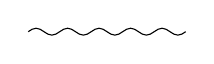
\begin{tikzpicture}
    \draw[decorate,decoration=wave] (0,0) -- (2,0) ;
  \end{tikzpicture}
\end{example}

\subsubsection{For Module Writers}
The \chemmodule{tikz} module provides some macros for common \TikZ\
functions.  This allows to use expl3's powerful function variants for
expansion control.

\begin{commands}
  \command*{c_chemmacros_other_colon_tl}
    A constant tokenlist which contains a colon with category code~12 (other).
    This is useful since \TikZ\ sometimes expects an other colon and in an
    expl3 programming environment \code{:} has category code~11 (letter).
  \command*{chemmacros_tikz_picture:nn}[ \marg{options} \marg{code}]
    Defined as \verbcode+\tikzpicture[{#1}] #2 \endtikzpicture+.
  \command*{chemmacros_tikz:nn}[ \marg{options} \marg{code}]
    Defined as \verbcode+\tikz[{#1}]{#2}+.
  \command*{chemmacros_tikz_draw:n}[ \marg{options}]
    Defined as \verbcode+\draw[{#1}]+.
  \command*{chemmacros_tikz_node:n}[ \marg{options}]
    Defined as \verbcode+\node[{#1}]+.
  \command*{chemmacros_tikz_shade:n}[ \marg{options}]
    Defined as \verbcode+\shade[{#1}]+.
  \command*{chemmacros_tikz_shadedraw:n}[ \marg{options}]
    Defined as \verbcode+\shadedraw[{#1}]+.
  \command*{chemmacros_tikz_node_in_draw:n}[ \marg{options}]
    Defined as \verbcode+node[{#1}]+.
\end{commands}

% TODO

\subsection{The \chemmodule*{xfrac} Module}\label{sec:xfrac-module}

The \chemmodule{xfrac} module loads the package
\pkg{xfrac}~\cite{bnd:l3packages}.  For the following explanations it will be
helpful if you know about said package and how it works first.  This module is
a support module that defines the macro
\begin{commands}
  \command{chemfrac}[\oarg{type}\marg{numerator}\marg{denominator}]
    \meta{type} can either be \code{text} or \code{superscript}.
\end{commands}
This macro calls a certain instance of the \pkg{xfrac} \code{text} template,
depending on the option \meta{type} and the current font family.  If used
\cs{chemfrac} looks if an instance
\begin{center}
  \code{chemmacros-frac-\cs*{f@family}-\meta{type}}
\end{center}
exists.  If yes this instance is used, if no the instance
\code{chemmacros-frac-default-\meta{type}} is used.  The \code{default}
instances are the same as the ones for \code{cmr}.

\begin{table}
  \centering
  \newcommand*\showfrac[1]{%
    \code{#1} &
    \fontfamily{#1}\selectfont
    \chemfrac[text]{2}{3} &
    \fontfamily{#1}\selectfont
    \chemfrac[superscript]{2}{3}%
  }
  \caption{Predefined \chemmodule{xfrac} \code{text} instances.}
  \label{tab:xfrac}
  \begin{tabular}{llcc}
    \toprule
      \bfseries font family & \bfseries text & \bfseries superscript \\
    \midrule
      \showfrac{cmr} \\
      \showfrac{lmr} \\
      \showfrac{LinuxLibertineT-TLF} \\
      \showfrac{LinuxLibertineT-TOsF} \\
    \bottomrule
  \end{tabular}
\end{table}

The \chemmodule{xfrac} module defines instances some font families, they are
listed and demonstrated in table~\vref{tab:xfrac}.  The \code{superscript}
type fractions \emph{look} larger than the \code{text} types.  The reason is
that the \code{superscript} types are typically used with a smaller font size.
Let's take a look at an example where both instances are used:
\begin{example}[side-by-side]
  \chemsetup[redox]{pos=top}
  \code{superscript}:
  \ch{"\ox{1/3,I}" {}3+}

  \chemsetup[redox]{pos=side}
  \code{text}: \ox{1/3,I3+}

  \huge
  \chemsetup[redox]{pos=top}
  \code{superscript}:
  \ch{"\ox{1/3,I}" {}3+}

  \chemsetup[redox]{pos=side}
  \code{text}: \ox{1/3,I3+}
\end{example}

If you define instances for other families please feel free to submit them to
me (see section~\vref{sec:submitting-module}) so they can be added to the
\chemmodule{xfrac} module.

\appendix
\part{Appendix}
\section{Own Modules}\label{sec:own-modules}
\subsection{How To}

If you have additional functionality which you think might be useful as a
\chemmacros\ module then you can easily write one yourself.  The module must
be a file in a path where \TeX\ can find it following a certain naming
scheme.  The file for a module \chemmodule*{foo} \emph{must be named}
\code{chemmacros.module.foo.code.tex}.

\begin{commands}
  \command{ChemModule}[\sarg\marg{name}\marg{description}\oarg{minimal
    compatibility version}]
    Register module \meta{name}.  The optional argument \meta{minimal
      compatibility version} ensures that this module is only loaded if the
    option \option{compatibility} has a high enough version number.  If it is
    omitted the module can be loaded in each version~5.0 or higher.
\end{commands}

The first line in the file then should look similar to this:
\begin{sourcecode}
  \ChemModule{foo}{2015/07/14 description of foo}
\end{sourcecode}
This registers module \chemmodule*{foo} which means \chemmacros\ will accept
this file as a valid module.

Since \chemmacros\ is written using expl3 \cs{ChemModule} starts an expl3
programming environment.  If you don't want that but rather want to write your
module using traditional \LaTeXe\ methods then use the starred variant:
\begin{sourcecode}
  \ChemModule*{foo}{2015/07/14 description of foo}
\end{sourcecode}
In both variants \code{@} has category code~11 (letter).

Since new modules very likely might rely on code provided first in a certain
version of \chemmacros\ you might want to make sure that your module only is
loaded when the compatibility mode is high enough to provide the features you
want:
\begin{sourcecode}
  \ChemModule{foo}{2015/10/14 description of foo}[5.2]
\end{sourcecode}

You should be aware that your module \emph{will not be loaded} with
\verbcode+\usechemmodule{all}+! The pseudo-module \chemmodule{all} contains a
manually maintained list of the modules that are loaded by it.

If you decide to write your module \chemmodule*{foo} using expl3 and add
options you want to be able to set using
\cs{chemsetup}\Oarg{foo}\marg{options} please make sure you define (and set)
them with the following macros:
\begin{commands}
  \command*{chemmacros_define_keys:nn}[ \marg{module} \marg{key definitions}]
    Define l3keys options for the module \meta{module}.  This is a wrapper for
    \cs*{keys_define:nn} \Marg{chemmacros/\meta{module}} \marg{key
      definitions}.
  \command*{chemmacros_set_keys:nn}[ \marg{module} \marg{input}]
    Sets l3keys options for the module \meta{module}.  This is a wrapper for
    \cs*{keys_set:nn} \Marg{chemmacros/\meta{module}} \marg{input}.
\end{commands}
Also (\emph{especially if you consider submitting the module, see
  section~\vref{sec:submitting-module}}) please follow the expl3 naming
conventions for variables and functions, \ie, use \code{chemmacros} as expl3
module name:
\begin{sourcecode}
  \tl_new:N \l__chemmacros_my_internal_variable_tl
  \tl_new:N \l_chemmacros_my_public_variable_tl
  \cs_new:Npn \__chemmacros_my_internal_function:n #1 { ... }
  \cs_new_protected:Npn \chemmacros_my_public_function:n #1 { ... }
  \NewDocumentCommand \publicfunction {m}
    { \chemmacros_my_public_function:n {#1} }
\end{sourcecode}
You will find more details on the naming conventions in \code{interface3.pdf}
which most likely is available on your system:
\begin{bash}
  texdoc interface3
\end{bash}
If you haven't read section~\vref{sec:base-module} about the \chemmodule{base}
module, yet, please have a look.  There some macros for module writers are
described.  Also other modules define macros for module writers which may be
useful.

\subsection{Submitting a Module}\label{sec:submitting-module}

If you have written a module and feel it might be useful for other users
please feel free to contact me and submit the module.  I will surely take at
look at both functionality and code and if I feel that it adds value to
\chemmacros\ I will add it to the package.  Requirement for this is that the
module is licensed with the \LPPL\ (v1.3 or later) and that I take over
maintenance (according to the \enquote{maintainer} status of the \lppl).

Please do \emph{not} submit your module via pull request but send me the files
directly.  In the best case you also have a short piece of documentation.

\section{Suggestions, Bug Reports, Support}\label{sec:sugg-bug-reports}

\paragraph{Support}
If you need support or help with anything regarding \chemmacros\ please use
the usual support forums
\begin{itemize}
  \item \url{http://www.golatex.de/} or
  \item \url{http://texwelt.de/wissen/} if you speak German,
  \item \url{http://www.latex-community.org/forum/} or
  \item \url{http://tex.stackexchange.com/} if you speak English
\end{itemize}
or go the \emph{dedicated support forum}
\begin{itemize}
  \item \url{http://www.mychemistry.eu/forums/forum/chemmacros/}
\end{itemize}
where you can be sure that I will see the question.
  
\paragraph{Suggestions}
If you have any suggestions on how \chemmacros\ could be improved, adding
missing features \etc, please feel free to contact me via
\email{contact@mychemistry.eu}.

\paragraph{Bug reports}
If you find any bugs, \ie, errors (something not working as described,
conflicts with other packages, \ldots) then please go to
\url{https://github.com/cgnieder/chemmacros/issues/} and open a new issue
describing the error including a minimal working example.

\end{document}
